\documentclass[sigplan,review,twocolumn,anonymous]{acmart}
\usepackage{graphicx}
\usepackage{subfig}
%Removing the geometry package used for Tighter Format
%\usepackage{geometry}
%\usepackage{times}
\usepackage{textcomp}
\usepackage{multirow}
\usepackage{framed}
\usepackage{amsmath}
\usepackage{listings}
\usepackage{comment}
\usepackage{microtype}
\usepackage[noend]{algpseudocode}
\usepackage[nothing]{algorithm}
% \usepackage[hyphens]{url}
\PassOptionsToPackage{hyphens}{url}
\usepackage{hyperref}
%\usepackage{hyperref}
\usepackage{enumitem}
\usepackage{amssymb}
\usepackage{tabularx}
\usepackage[normalem]{ulem}
%Used only for breaking hypenated URLs
\usepackage{etoolbox}
\gappto{\UrlBreaks}{\UrlOrds}
%

\hypersetup{breaklinks=true}

\urlstyle{same}

%\usepackage[activate={true,nocompatibility},final,tracking=true,kerning=true,spacing=true,factor=1100,stretch=20,shrink=20]{microtype}


% \newcommand{\submissionnumber}{144}
% \newcommand{\sysname}{Il\'uvatar}
\newcommand{\D}{\emph{D}}
\newcommand{\Dmax}{\emph{D\_max}}
\newcommand{\T}{\emph{T}}
\newcommand{\VT}{\emph{VT}}
\newcommand{\GlobVT}{\emph{Global\_VT}}
\newcommand{\FinVT}{\todo{REMOVE: finish\_vt}}
% \newcommand{\QName}{MQ-FLQ}
% \newcommand{\QNameFull}{Multi-Queue Fair \& Local Queuing}
\newcommand{\QName}{MQFQ-Sticky}
\newcommand{\QNameFull}{\QName}
\newcommand{\batch}{\texttt{Batch}}
\newcommand{\naive}{\texttt{FCFS Naïve}}
\newcommand{\fcfs}{\texttt{FCFS}}

% \usepackage{tikz}

% \RequirePackage[normalem]{ulem}
% \RequirePackage{color}\definecolor{RED}{rgb}{1,0,0}\definecolor{BLUE}{rgb}{0,0,1}
\providecommand{\DIFadd}[1]{{\protect\color{blue}\uwave{#1}}}
\providecommand{\DIFdel}[1]{{\protect\color{red}\sout{#1}}}
%DIF SAFE PREAMBLE
\providecommand{\DIFaddbegin}{}
\providecommand{\DIFaddend}{}
\providecommand{\DIFdelbegin}{}
\providecommand{\DIFdelend}{}
%DIF FLOATSAFE PREAMBLE
\providecommand{\DIFaddFL}[1]{\DIFadd{#1}}
\providecommand{\DIFdelFL}[1]{\DIFdel{#1}}
\providecommand{\DIFaddbeginFL}{}
\providecommand{\DIFaddendFL}{}
\providecommand{\DIFdelbeginFL}{}
\providecommand{\DIFdelendFL}{}
%DIF END PREAMBLE EXTENSION ADDED BY LATEXDIFF

\def\Section {\S}

\newcommand{\squishlist}{
 \begin{list}{$\bullet$}
  { \setlength{\itemsep}{0pt}
     \setlength{\parsep}{3pt}
     \setlength{\topsep}{3pt}
     \setlength{\partopsep}{0pt}
     \setlength{\leftmargin}{1.5em}
     \setlength{\labelwidth}{1em}
     \setlength{\labelsep}{0.5em} } }
	
\newcommand{\squishlisttwo}{
 \begin{list}{$\bullet$}
  { \setlength{\itemsep}{0pt}
     \setlength{\parsep}{0pt}
    \setlength{\topsep}{0pt}
    \setlength{\partopsep}{0pt}
    \setlength{\leftmargin}{2em}
    \setlength{\labelwidth}{1.5em}
    \setlength{\labelsep}{0.5em} } }

\newcommand{\squishend}{
  \end{list}  }

% \newcommand{\squishenum}{
%   \begin{enumerate}{$\bullet$}
%     { \setlength{\itemsep}{0pt}
%       \setlength{\parsep}{0pt}
%       \setlength{\topsep}{0pt}
%       \setlength{\partopsep}{0pt}
%       \setlength{\leftmargin}{2em}
%       \setlength{\labelwidth}{1.5em}
%       \setlength{\labelsep}{0.5em} } }
  
% \newcommand{\squishenumend}{
%   \end{enumerate}  }

\newcommand{\alert}[1] {\textcolor{red} {\textsc{#1}}}

\newcommand{\myfbox}[1] {\noindent \fbox{\parbox{0.5\textwidth} {#1}}}

\newcommand{\mhead}[1] {\noindent \textbf{#1.}}

\newcommand*\mean[1]{\overline{#1}}

\newcommand{\eat}[1]{}

\newcommand{\compresslist}{%
  \setlength{\itemsep}{1pt}%
  \setlength{\leftmargin}{1.5em}
  \setlength{\labelwidth}{1em}
  \setlength{\parskip}{0pt}%
  \setlength{\parsep}{0pt}%
%  \setlength{\itemindent}{-10pt}%
}

\newcommand{\myfigspace}[0]{-0.3cm}
\newcommand{\bigfigspace}[0]{-0.9cm}
\newcommand{\captionspace}[0]{-0.25cm}
\newcommand{\subsecspace}[0]{-0.1cm}
\newcommand{\largesubsecspace}[0]{-0.38cm}

\newcommand\prat[1]{\textcolor{red}{(Prateek: #1)}}

\newcommand{\quotes}[1]{``#1''}
\newcommand{\todo}[1]{\textcolor{orange}{TODO: #1}}
\newcommand{\alex}[1]{\textcolor{blue}{Alex: #1}}
% https://tex.stackexchange.com/a/7045
\newcommand*\circled[1]{\tikz[baseline=(char.base)]{
            \node[shape=circle,draw,inner sep=2pt] (char) {#1};}}


\newcommand{\funcname}[1]{\texttt{#1}}
\renewcommand\footnotetextcopyrightpermission[1]{}
% Optional: Remove the ACM reference between the abstract and the main text.
\setcopyright{none}
\settopmatter{printacmref=false}
\acmConference{}{}{}
\acmPrice{}
\acmISBN{}
\acmDOI{}
\acmYear{}
\acmMonth{}

\settopmatter{printfolios=true,printacmref=false}
\acmSubmissionID{\submissionnumber}

\begin{document}
%-------------------------------------------------------------------------------

%\title{Any Function, Any GPU: Acceleration and Multiplexing for Serverless Systems}
%\title{Black-Box GPU Acceleration and Multiplexing for Serverless Systems}
\title{Opportunistic GPU Acceleration for Serverless Functions}

%don't want date printed
\date{}

% make title bold and 14 pt font (Latex default is non-bold, 16 pt)
\author{}

\begin{abstract}
Hardware accelerators like GPUs are now ubiquitous in data centers and edge computing, but are not fully supported by common cloud abstractions such as serverless Functions as a Service (FaaS).
Many popular and emerging FaaS applications such as machine learning and scientific computing  can benefit from GPU acceleration.
However, FaaS frameworks (such as OpenWhisk) are not capable of providing this acceleration because of the design mismatch between the GPU usage and FaaS programming model, which requires virtualization and sandboxing of each function, and must support highly dynamic and heterogeneous functions. 

This paper presents the design and implementation of a FaaS system for heterogeneous hardware, which provides hybrid computing capabilities for general, black-box functions.
We show how data and code locality determines GPU function performance, and translate principles from I/O scheduling such as fair queuing and anticipatory scheduling, to GPUs. 
On real-world FaaS workloads, our fair-queuing scheduling can reduce latency by more than 5x compared to FCFS and batch-oriented scheduling. 
Our scheduler-integrated memory movement optimizations significantly reduce GPU cold-starts, reducing function latency by more than two orders of magnitude, allowing FaaS operators to provide opportunistic acceleration and leverage antiquated GPUs. 

%we show that even obselete GPUs can reduce function latency by more than 2x compared to pure CPU execution. 

\end{abstract}

\maketitle 

%\thispagestyle{empty}

%%%%%%%%%%%%%%%%%%%%%%%%%%%%%%%%%%%%%%%%%%%%%%%%%%

%\vspace{-0.3cm}

\section{Introduction}

Function as a Service (also called FaaS or serverless computing) is one of the fastest growing abstractions in cloud computing today with usage increasing by 2x in the past two years alone~\cite{wen2023rise}.
% Users create self-contained \textit{functions} whose lifecycle is orchestrated by the FaaS provider.  
Users are enticed by its dynamic scaling, low cost, and ease of management, as the lifecycle of self-contained \textit{functions} is orchestrated by the FaaS provider.
% Cloud providers benefit because functions use ephemeral resources unlike traditional virtual machines (VMs) and the provider has find-grained control over scheduling and placement.
Cloud providers leverage the ephemeral nature of functions into fine-grained control over scheduling, placement, and resource allocation.

% 1)
Current FaaS applications are limited by the capabilities exposed by providers, mostly consisting of short-running functions~\cite{shahrad2020serverless} using limited compute.
% Functions are given limited CPU resources and have no way efficient of coordinating with one another, precluding classic parallel computing.
Providers have not exposed GPUs or other parallel processing paradigms to their serverless platforms, a need for which is growing as users migrate new, intensive, workflows to cloud FaaS.
These applications see a \emph{minimum} 2.5x throughput improvement when accelerated, strong encouragement to enable such devices in serverless platforms.

% 2-3)
Accomplishing this transition requires the control plane to address several resource management problems.
Achieving high device utilization and low latency require device multiplexing~\cite{pemberton2022kernel, ng2023paella, fingler2022dgsf, gu2023fast}, but unmodified functions preclude such sharing of GPU resources.
% To make matters more complicated, GPU resources are managed by an esoteric device driver that isn't controllable by the OS.
Once a function is given access to the GPU, it can allocate the entire memory range or hog compute in a run-to-completion model.
% Idle periods mean allocated resources on the GPU are blocked off, other functions being unable to use them for their executions.
% Removing containers to release held resources results in heavy churn and increased latency from the repeated container initialization.
Swapping functions requires starting a new container, costing several seconds on the critical path, making the well-known \quotes{cold start} problem of FaaS an even larger latency bottleneck.
% We avoid cold starts by being the first to enable GPU keep-alive~\cite{faascache-asplos21} policies via GPU resource multiplexing.
Avoiding cold starts (i.e. a warm start) to get viable performance requires enabling GPU keep-alive~\cite{faascache-asplos21} policies via GPU resource multiplexing.

\begin{comment}
Machines used to host FaaS systems are expected to serve thousands of unique functions with low latency.
This is accomplished by running user function code inside a container (or VM), then keeping the container in memory but idle for future uses. 
A na\"ive adaption of this to the GPU problem would assign an entire GPU to each container for its lifetime.
Unfortunately an idle container then wastes GPU resources, and the limited number of GPUs per server leads to churn when we need to create a new container for another function.
% but this causes low utilization and high turnover when going to run a new function.
Virtualization for these devices exists, provisioning fixed slices of GPU resources to containers that they then have exclusive access to.
% This also results in low utilization, as nothing else can use that section when it is idle, and also limits the resources available to give to any one function that might take advantage of them.
While allowing more containers to exist concurrently, this solution does not address idleness and introduces a new limitation by reducing the maximum allocation any single function is allowed to make.
\end{comment}
  
% 4-6)
Multiplexed resources are not a performance panacea: the platform must now contend with function fairness and locality.
% The FaaS control plane must also guarantee that all functions will run in a timely and fair manner.
% GPUs must also be shared temporally 
Optimal performance is achieved by running one function repeatedly, as its data dependencies will be available on-device.
Yet a popular function can easily starve others of device time and violate fairness guarantees if not eventually blocked.
% Temporal GPU sharing between the highly heterogeneous serverless workloads must be balanced with execution \quotes{locality}.
New queuing policies tailored to the unique scenario of GPU-serverless computing must be designed to ensure fairness while maintaining high throughput.
% Warm hits, i.e. executing using an already existing container, have up to 100x lower latency compared to their cold counterparts.
% Such execution \quotes{locality} can only come 
% want warm starts.
% locality good -> 'batching'.
% but need spatial/temporal multiplexing as well.

% 7
Previous research work into enabling GPU acceleration in FaaS has focused on ML inference~\cite{pemberton2022kernel, ng2023paella, fingler2022dgsf, gu2023fast}; understandable given its popularity.
These approaches have abandoned the black-box nature of FaaS in favor of extremely fine-grained control of GPU usage and scheduling.
Supporting functions of all types is critical, as more use cases like scientific computing~\cite{kumanov2018serverless,hung2019rapid}, video encoding~\cite{ao2018sprocket, zhang2019video}, and optimization problems~\cite{aytekin2019harnessing,werner2018serverless,shankar2020serverless}, migrate to the platform.
% Our work uniquely enables all these to run natively with minimal overhead.
% Custom solutions have been proposed~\cite{}, but rely on targeted workloads or bespoke platforms, a general-purpose approach is needed.

% 7)
Given these known problems, in this work we seek to answer several research questions:
\begin{enumerate}[leftmargin=*]
  % \item Can we provide GPU acceleration to black-box, unmodified, serverless functions?
  % \item How can GPU support be integrated into high-performance FaaS control planes?
  \item Can we provide GPU acceleration to black-box, unmodified, serverless functions?
  \item Can we multiplex GPU resources between functions in a low overhead manner?
  \item How do we balance locality, fairness, and performance in the face of heterogeneous functions?
  % \item Is this possible without the cost of full virtualization?
\end{enumerate}
% \todo{Better RQs to frame novelty}

In this work, we propose and designed a series of techniques and policies that resolve all of these issues.
They enable black-box serverless functions to utilize GPUs for acceleration while concurrently sharing its resources.
We built our system on top of the \sysname~platform~\cite{fuerst2023iluvatar}, utilizing Nvidia's integration with Docker~\cite{docker-main}. %, but is generic to any accelerator or isolation system.
Importantly, they don't rely on specific hardware or software versioning support, and work on heterogeneous hardware regardless of age or capability. 

% \mhead{RQ1}
Starting from the lowest level component, we interpose an intercept shim between function code and the GPU driver.
Using this, we capture all memory allocation calls and transform them into Unified Virtual Memory (UVM)~\cite{nvidia-uvm} calls.
UVM memory allows applications to allocate beyond the device limits, letting the driver use host memory as swap space, migrating memory on demand. 
Once all allocations are converted to UVM memory, we use the shim to move memory between host and device under direction from the control plane.

% \mhead{RQ2}
Controlling memory positioning allows us to both oversubscribe device memory and keep containers warm while other functions execute on the GPU.
To enable multiple functions to run concurrently, a new queuing policy is required that better matches the new device's capabilities and workload characteristics.
We accomplish this with a modified implementation of a Mutli-Queue Fair Queue (MQFQ)~\cite{hedayati2019multi}, which prevents starvation, scales invocations across multiple GPUs, and minimizes execution overhead.
To prevent contention interference, we monitor device utilization using NVML~\cite{nvml} and track memory usage to throttle invocations.

With these controls we improve function latency by orders of magnitude over previous solutions and expand the pool of serverless applications.
In short, this work proposes the following enhancements to serverless computing:
\begin{enumerate}[leftmargin=*]
  \item We create a custom driver that intercepts function allocation calls to multiplex device memory.
  \item With no limit on device memory, we can keep idle containers resident, creating the first warm pool of GPU containers.
  \item Our memory management techniques allow us to reduce device pressure from idle functions, mitigating overcommitment overhead.
  \item We design a queuing policy that enables concurrent execution while ensuring fairness under heterogeneous workloads.
  % \item W
  % \item Benchmark suite of GPU-enabled serverless functions, including many non-machine learning applications.
\end{enumerate}

This paper is ordered as follows.
Section~\ref{sec:bg} covers background of serverless work and GPU virtualization.
Our motivation behind work is explained in detail in Section~\ref{sec:motiv}.
Section~\ref{sec:design} details our design of queuing, memory control, and resource management.
We examine the implementation of these pieces in Section~\ref{sec:impl}.
Lastly, Section~\ref{sec:eval} shows the effectiveness of our systems with a thorough experiment suite.
 

\section{Background and Motivation}
\label{sec:bg}

\begin{comment}
\subsection{Providing Functions as a Service}

Serverless computing entails executing snippets of user code, usually in an event-driven manner, inside protected and isolated sandboxes~\cite{serverless-cacm-21}.
For users, serverless functions offer many features such as elastic scaling and scale-to-zero, making cloud-native applications easier to develop and deploy. 
% As a result, FaaS has emerged as a common abstraction for a wide range of cloud services such as orchestration and workflows, IoT, machine learning and data analytics pipelines, scientific computing, etc. 
The FaaS \emph{provider} usually runs a \emph{control plane} such as OpenWhisk and OpenFaaS (or proprietary ones in the case of popular services like Amazon Lambda~\cite{aws-lambda}), for handling the scheduling, scaling, load-balancing, resource limiting, and accounting for each invocation. 

From the FaaS control plane's perspective, the popularity and diversity of FaaS workloads makes these tasks particularly challenging, and can add several dozen milliseconds of latency in orchestrating function invocations~\cite{cvetkovic2024dirigent, fuerst2023iluvatar, serverless-cluster-cost}.
Because of the richness of their usecases, function workloads are highly diverse with a range of several orders of magnitude in all dimensions.
For example, both Azure~\cite{shahrad2020serverless} and Alibaba~\cite{luo2021characterizing} workloads indicate that the inter-arrival-times can range from 0.1s to hours, the execution times can range from milliseconds to minutes, and the memory footprint from 100 MB to 5 GB. 
From the FaaS control plane point of view, an invocation is a \quotes{black-box} containerized task with known resource limits (such as the number of allocated CPUs and memory size).
Function resource usage is typically similar across invocations, and control planes also use these estimates for implementing advanced policies for keep-alive~\cite{roy2022icebreaker,faascache-asplos21}, placement, etc. 
\end{comment}

\subsection{Why GPU Acceleration for Functions}

%1. Many applications benefit
%2. GPU hardware present on many servers anyways. Thus need the opportunistic acceleration. 
\begin{comment}
\mhead{Serverless Use Cases}
The number of serverless use cases than use or can benefit from acceleration is continuously growing.
Encoding of videos~\cite{ao2018sprocket, zhang2019video} and analytics on live video streaming~\cite{romero2021llama, risco2021gpu} are ideal for both FaaS scaling and internal application parallelism. 
% Machine learning in all its forms has made its way into the serverless research.
% Commonly to make scheduling decisions for containers~\cite{balaji2021fireplace} or resource allocation to them~ \cite{mvondo2021ofc,eismann2021sizeless}.
Machine learning inference has need for low-latency results, and has seen much work in serverless~\cite{yang2022infless, ali2022optimizing, ali_batch_2020}, and can achieve lower latency with acceleration.
% And finally are works that do training, taking advantage of the serverless scaling~\cite{wang2019distributed, gimeno2022mlless, xu2021lambdadnn}.
%
The exposure of supercomputing resources to run scientific workloads by~\cite{funcx_hpdc_20} highlights the demand for parallelization of functions.
Such science workloads vary from biomedical research~\cite{kumanov2018serverless,hung2019rapid}, linear algebra~\cite{werner2018serverless,shankar2020serverless}, to optimization algorithms~\cite{aytekin2019harnessing}.
\end{comment}

\begin{table}
  \centering
  \caption{Latencies (in seconds) for GPU and CPU \textbf{W}arm and \textbf{C}old functions.}
  \label{tab:gpu-cpu}
  % \begin{center}
  \begin{tabular}{lccc}
    \hline
    Function & GPU [\textbf{W}] & CPU [\textbf{W}] & GPU [\textbf{C}] \\
    \hline
  Imagenet [ML] & 2.253 & 5.477 &     8.581 \\
  Roberta [ML] & 0.268 & 5.162 &     16.374 \\
  Ffmpeg [Video] & 4.483 & 32.997 &     12.044 \\
  FFT [HPC] & 0.897 & 11.584 &     2.648 \\
  % Eos & 0.017 & 0.045 & 2.66x \\
  Isoneural [HPC] & 0.026 & 0.501 &     2.586 \\
  % Lavamd & 1.989 & 15.199 & 7.64x \\
  Lud [Rodinia] & 2.050 & 70.915 &     2.125 \\
    Myocyte [Rodinia] & 2.784 & 39.277 &      2.145 \\
  Needle [Rodinia] & 1.979 & 144.639 &     2.292 \\
  Pathfinder [Rodinia] & 1.472 & 134.358 &     1.997 \\
  % Srad & 3.893 & 119.759 & 30.77x \\
  \end{tabular}
% \end{center}
\end{table}

% One of the first works to integrate GPUs is~\cite{naranjo2020accelerated} using rCUDA~\cite{duato2010rcuda} to connect disaggregated GPUs in a cluster to containers.
% It only looks at the performance affect on individual function invocations, not exploring the resource management, queuing, or heterogeneous load issues in FaaS.
% DGSF~\cite{fingler2022dgsf} combines disaggregation and API remoting to improve utilization, and does load-balancing between GPUs on the compute node.


Many applications that have adopted FaaS for its on-demand scaling also benefit from GPU acceleration, as shown by Table~\ref{tab:gpu-cpu}, where we compare the execution times of functions using an NVidia V100 GPU and an Intel Xeon Gold 3.2 GHz CPU.
CPU functions are allocated one CPU core, and GPU functions can use the entire accelerator.
Machine learning inference tasks such as Imagenet and Roberta see a 3x and 20x reduction in latency compared to a warm CPU container. 
Video encoding via \emph{ffmpeg}, which is one of the most popular functions on AWS Lambda~\cite{aws-netflix}, can also leverage specialized hardware found in most GPUs for a 7x speedup. 
Scientific computing has started to be used in FaaS~\cite{john_sweep_2019,mocskos_faaster_2018,werner2018serverless,shankar2020serverless}, and also benefits from GPU acceleration for its common primitives such as FFT.
%One such ubiquitious algorithm, Fast Fourier Transform (FFT), sees 13x improvement, and larger, complete applications (Needle, Pathfinder, etc.) are 80-90x faster with acceleration. 


Thus a large class of FaaS workloads are potentially amenable to GPU acceleration.
The serverless abstraction allows decoupling of computation from its location, and prior work has investigated the use of remote disaggregated GPUs for FaaS~\cite{naranjo2020accelerated,fingler2022dgsf}, and providing acceleration as a service~\cite{varghese2015acceleration,du2022serverless}.
%These prior efforts have focused on the virtualization of accelerators through new mechanisms and abstractions, and often for specialized workloads such as ML inference.
%We focus on a higher level of abstraction, and develop scheduling policies for providing GPU acceleration \emph{at scale} which can be integrated as part of a high-performance FaaS control plane.
Serverless functions in public cloud with enabled GPUs have started to appear~\cite{azure-gpu-function,alibaba-gpu-function}, but are far from ideal.
These use GPU-passthrough techniques~\cite{alibaba-gpu-noshare}, which statically allocate hardware and have low utilization, and sometimes one must even self-host the hardware~\cite{azure-gpu-function}.

% \todo{Add refs for azure and alibaba gpu functions and describe how they are limited/different. See \cite{sage_zhao_towards_2024} for these refs.}

\subsection{GPU Programming Model}
%TODO: Integrate with previous (gpu support for functions)

Applications cannot usually manipulate GPUs directly, and must use a manufacturer-provided driver for all operations.
Host programs launch \emph{kernels} which execute a code block with given memory inputs and a number of parallel threads to use.
Multiple kernels can be launched concurrently, with the device handling scheduling of kernels and threads internally.
Kernels run until completion, with execution time varying widely depending on the number of threads, input size, and complexity of the code being run. 
Traditionally, programs manually move data between the host and device (using \funcname{cuMemAlloc} for instance).
Virtualizing GPU memory (by using CUDA's Unified Virtual Memory (UVM)~\cite{nvidia-uvm}) allows memory overcommittment, which is important for supporting high degrees of multiplexing.
% Programs allocate memory using \funcname{cuMemAllocManaged} instead of \funcname{cuMemAlloc}, and the device driver moves memory between the device and host in response to usage and memory pressure.
%When using \funcname{cuMemAllocManaged}, the same memory pointer can be used on both host and device, and the driver is responsible for data migration and coherency.
%This capability is also used by UVM to allow over-subscription of memory, as it will move data pages around on-demand, using host memory as \quotes{swap} space. 
%We integrate our control plane with UVM to actively oversubscribe memory, allowing many function containers to remain warm on a device without interference, dramatically reducing cold starts. 

For multiplexing functions on GPUs, the naive approach entails fully assigning the GPU to a function. 
Because functions are short-lived (at most a few minutes), we can use the GPU in an FCFS run-to-completion model. 
However, this leads to poor GPU utilization since functions are often small and will not use all GPU resources, and also highly detrimental for function latency due to cold-starts, as we explain in the next section. 
A typical FaaS server runs 10--50 functions concurrently, and thus even if a small fraction of them can benefit from GPU acceleration, an immediate need arises for multiplexing the GPU to run multiple functions concurrently. 
However, GPUs have conventionally been designed for high throughput computation for a single long-running application, which is reflected in their hardware architecture and software stacks.
The performance-first focus has also resulted in many cross-layer optimizations which make multiplexing and virtualization challenging. 


% , regardless of the function it is for.
% The amount of GPU memory and compute usable by a process can be specified at process launch time, and is fixed thereafter.
% Importantly, support for MPS features varies between hardware versions, and only the newest devices have resource management features.
% Both spatial approaches have drawbacks that render them unsuitable for FaaS.

% Resource partitioning, a new container must be spun up with the large overhead that entails.
% MPS does not enable oversubscribing limited device memory, and the inability to truly isolate processes from one another makes it a poor candidate for FaaS.
% Both spatial sharing schemes do not allow variable resource allocations, requiring a container cold start to change allocations.
% Neither enable oversubscription of limited device memory, 


\begin{comment}
\mhead{Memory Multiplexing}
Limitations caused by requiring driver interaction to control the device makes it a challenge to multiplex memory.
Virtualization approaches~\cite{yu2019automatic, hong2017gpu} must duplicate application state in host memory, and allocate/de-allocate all resources when switching between applications.
Kernel level schedulers~\cite{ng2023paella,pemberton2022kernel,strati2024orion} are able to manipulate and oversubscribe memory as any GPU application would, but violate the black-box principles we target.
Interposition and disaggregation techniques~\cite{duato2010rcuda,fingler2022dgsf} allow for true multiplexing similar to our design, thanks to their level of control equal to that of a kernel scheduler while not being part of the actual application.
\end{comment}

\section{Design Requirements and Key Challenges}
\label{sec:motiv}

Our work considers discrete and integrated GPUs, and our task is to provide \emph{opportunistic} GPU acceleration to functions that benefit from it.
We assume a classic, non-disaggregated hardware platform where the GPU functions can run locally. 
Due to the surge of ML workloads, discrete and integrated GPUs are a common feature in data center and even edge clusters. 
For example, the popular Nvidia Jetson Orin platform provides more than 60\% of its compute capabilities (FLOPS) in the integrated GPU.
% \todo{Check FLOPS}
Since FaaS is the common abstraction for supporting a wide range of applications, we seek a general-purpose \emph{black-box} solution which supports arbitrary functions on heterogeneous clusters, and preserves existing resource isolation guarantees. 
This requires us to support different GPU usage patterns, and prevent the use of application-specific performance optimizations (such as for ML inference). 
For the FaaS hardware, we make minimal assumptions in terms of feature availability, and assume that the underlying cluster is a mix of servers with different GPU types, and support both data center and edge computing devices. 
Given all these requirements, the performance objective is to increase server utilization by running functions on GPUs, and reducing the overall function latency of FaaS workloads. 
The above constraints imposed by black-box FaaS workloads and GPU multiplexing also restrict the space of mechanisms and optimizations, which lead to the challenges described below. 


%Yet any function with a dataset that exceeds these limits or a problem space that needs parallel computing for timely results cannot be served.

\subsection{Cold-starts for GPU Containers}

\begin{figure}
  \centering
  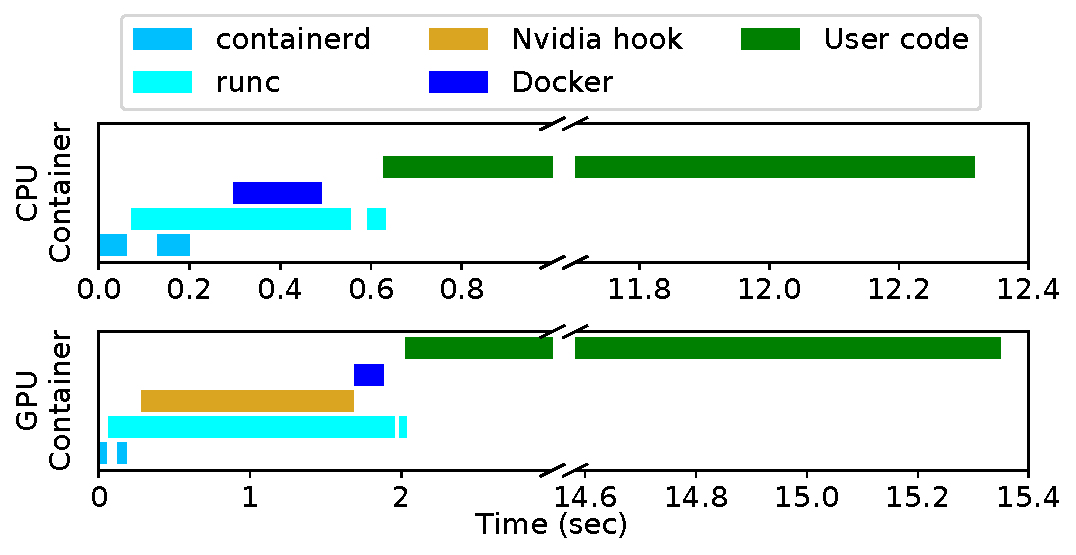
\includegraphics[width=0.9\textwidth]{./mqfq-final/graphs/coldstart/combined_timeline.pdf}
  \caption{Timeline of cold-starts of CPU (top) and GPU (bottom) function containers running TensorFlow inference code. 
    % Several additional seconds are caused by Nvidia runtimes and user code library loading.
    GPU initialization and code dependencies increase latency by three seconds.}
    \label{fig:cold-timeline}
% Gunicorn & library load time, no GPU:
% gunicorn: 0:00:11.688722
% Gunicorn & library load time, GPU:
% gunicorn: 0:00:13.320342
% nvidia: 0:00:01.399233
\end{figure}

Cold-starts due to sandbox creation and initialization are a well known performance problem for serverless functions~\cite{du2020catalyzer,lin_mitigating_2019,manner_cold_2018,mohan_agile_2019}.
We find that such cold starts are severely exacerbated by GPU containers, increasing latency by $1.1-75\times$ (Table~\ref{tab:gpu-cpu}).
A breakdown and comparison of these overheads for the ML inference function (using TensorFlow) is shown in Figure~\ref{fig:cold-timeline}.
For the GPU container (bottom figure), the Nvidia hook library adds more than 1.5 seconds of delay.
% , even before counting time taken by the application for initializing the GPU and loading specialized libraries.
% has the accelerator and spends roughly 1.5 seconds in an Nvidia library hook that performs kernel work to attach the GPU to the container.
User function code loads additional GPU libraries and dependencies, and its startup requires 1.5 additional seconds.
% lol not gonna do. TF does magic/BS loading of different stuff when a GPU is detected.
% \todo{Add which libraries.}

\subsection{Tradeoffs in Locality, Throughput, and Fairness}

A common approach to alleviate cold starts is to keep the container warm~\cite{faascache-asplos21} in memory.
This is also applicable for GPU containers, but with additional challenges.
First, a warm container holds GPU memory which is much more limited (e.g., the V100 has 16 GB VRAM), which reduces keep-alive's effectiveness~\cite{faascache-asplos21}, and reduces the number of containers able to be kept warm.
Additionally, the number of concurrently executing functions should also be kept low to mitigate performance interference, which can be excessive from both compute~\cite{yamagiwa2009performance,phull2012interference} and data movement between host and device~\cite{yu2019automatic, hong2017gpu}.
This reduction in concurrency increases queue waiting times.
Finally, since function workloads are highly heterogeneous and dynamic, we must select the \quotes{active} functions carefully so as to balance fairness and throughput.
% The scheduling is also affected by the high cost of data movement between host and device~\cite{yu2019automatic, hong2017gpu}.


In other contexts, application switching costs have been reduced through batching.
For example, an ML inference task can be given multiple inputs simultaneously as a batch---significantly improving throughput and utilization~\cite{ali_batch_2020,yang2022infless,ali2022optimizing}.
%The inputs of multiple invocations are merged into one \emph{batch} by the control plane, computed together, and split apart to distribute results.
% Scientific applications among others are not amenable to batching, and for those that do, they require changing the FaaS paradigm.
Such specialized and white-box solutions eschew isolation by making assumptions about the workload, such as the ability to modify the function code and input/output processing. 
For a general FaaS service, we need to provide locality improvements using a black-box approach.


Maximizing for locality entails large batches, which increases latency for both the batched function and also the other functions due to monopolization of GPU resources.  
For heterogeneous and dynamic FaaS workloads, batching policies are also significantly more challenging outside more specialized workloads like inference-as-a-service.
For example, popular functions see $100\times$ the average number of invocations, which can cause the rest of the long tail of functions to have exacerbated waiting times in the queue, leading to unfairness. 
Thus, while locality is useful for performance, it may lead to unfairness. 

\subsection{GPU Multiplexing Mechanisms}

While many hardware- and software-level virtualization and multiplexing solutions exist, they are ill-suited for the highly dynamic and heterogeneous containerized function workloads.
%\mhead{Temporal Multiplexing}
The conventional approach is to dispatch multiple GPU compute kernels (corresponding to different functions) concurrently, and let the GPU driver and hardware manage the sharing of GPU compute cores and memory.
The GPU driver itself accepts individual compute \emph{kernels} from applications and has a device-internal scheduler which maps them to available compute blocks as they arrive. 
This is one of the main mechanisms behind classic GPU virtualization work~\cite{duato2010rcuda, yu2019automatic, hong2017gpu}, but comes with significant performance overheads~\cite{yu2017full}. 
These GPU virtualization approaches duplicate application state in host memory, and allocate/de-allocate all resources when switching between applications. 
% , and most target disaggregation~\cite{duato2010rcuda,fingler2022dgsf} or API imposition~\cite{yu2019automatic}.
% These support memory and compute sharing 


\emph{Application-specific} optimizations for scheduling and multiplexing of GPU kernels can be performed at several levels of the GPU software-hardware stack. 
% Replacement schedulers~\cite{mccoy2024gallatin} have been devised, as well as systems that schedule kernel launches from inside an application~\cite{strati2024orion}.
Kernel schedulers for domain-specific optimizations~\cite{strati2024orion,chen2017effisha,kim2020navigator,gu2023fast} have been designed to coordinate kernels from several applications to improve on device scheduler performance.
These operate only on compute kernels to prevent contention and assume active concurrent workloads are coordinated elsewhere to not exceed the device memory. 
% At the highest level, a process or job can be scheduled on a specific GPU and allowed to run to completion, accepting the application's arbitrary kernel launches. 
% As many workloads can't consume all available GPU resources, some schedulers control both kernel launches and device memory.
Application-optimized and integrated scheduling solutions have recently been developed~\cite{ng2023paella,pemberton2022kernel,strati2024orion}, which interpose on the application's kernel launches.
For example, the structure of ML inference applications can be used for injecting kernel preemption code into the applications via TVM transformations~\cite{han2022microsecond} for decreasing head of line blocking and improving GPU utilization.


%include manipulating and oversubscribing memory as they schedule kernel launches, but they violate the black-box principles we target by breaking apart the application to have tighter control.
%Interposition and disaggregation techniques~\cite{fingler2022dgsf,duato2010rcuda} allow for multiplexing memory and compute similar to our design, thanks to the level of control gained by replacing the GPU driver, and are black-box because they do not replace the actual application.


GPU compute cores and memory can also be \emph{spatially partitioned} across clients/kernels using more modern GPU virtualization functionality. 
% via virtualization that vary with different hardware generations.
% Virtualization passthrough of vGPUs~\cite{nvidia-passthrough} uses direct device assignment common to hardware virtualization, where a guest VM has total control of the device with no sharing. 
Nvidia MIG~\cite{nvidia-mig} (Multi-Instance GPU) pre-partitions device resources, and one or more of these virtualized GPU partitions can be assigned to a VM or container via direct device assignment.
However, the slices are of pre-determined sizes, making them ill-suited to fine-grained and dynamic workloads~\cite{li2022miso}. 
Similarly, Multi-Process Service~\cite{nvidia-mps} (MPS) allows multiple processes to make share the device concurrently and has been proposed for FaaS~\cite{gu2023fast}.
An MPS server and the hardware device perform resource partitioning based on configuration at application start time.
MPS is explicitly designed to let cooperative processes share GPU resources, and documentation specifies that it is intended to work with OpenMP/MPI applications~\cite{nvidia-mps}.
If any process fails and crashes, all processes connected to the MPS server will crash, meaning one faulty serverless function will break all functions using that GPU, which we have frequently experienced in our testing.

Thus, neither MIG nor MPS are suited for serving FaaS workloads.
Moreover, they are not uniformly available across GPUs---for example, Nvidia's Jetson IoT GPUs do not support MPS~\cite{jetson-no-mps}, and MIG support is only found in select GPUs after 2020 supporting Nvidia's Ampere architecture.
Our requirement is to support acceleration for GPUs which may not be state of the art and thus not support hardware assisted virtualization such as MIG or vGPUs.
Instead, we seek to interweave scheduling and multiplexing techniques to maximize fairness and throughput.



% The first proposal~\cite{naranjo2020accelerated} used Docker and only shows performance improvement against CPU runtimes, neither queuing nor any drawbacks from switching computation are considered. 
% Several examples~\cite{pemberton2022kernel,gu2023fast,ng2023paella} do schedule ML inference tasks and GPU resources for high GPU utilization, but do so by breaking apart each function to control kernel launches, thereby preclude whole classes of applications from running.



%%% Local Variables:
%%% mode: latex
%%% TeX-master: "paper"
%%% End:


%\vspace*{\subsecspace}
\section{Design: Scheduling GPU Functions}
\label{sec:design}

The main new contribution and component of our hybrid serverless computing platform is the scheduler for GPU functions, which we describe in this section. 
The different hardware and workload model of GPUs requires a different approach to scheduling as compared to conventional CPU function scheduling. 
To tackle these challenges, we first show that fair queuing as used in I/O scheduling can be a useful framework for GPU scheduling (Section~\ref{sec:d:mqfq}), then describe the GPU-specific scheduling (Section~\ref{sec:mq}) and memory management optimizations (Section~\ref{sec:design-cont-shim}). 

\begin{figure}
  \centering
  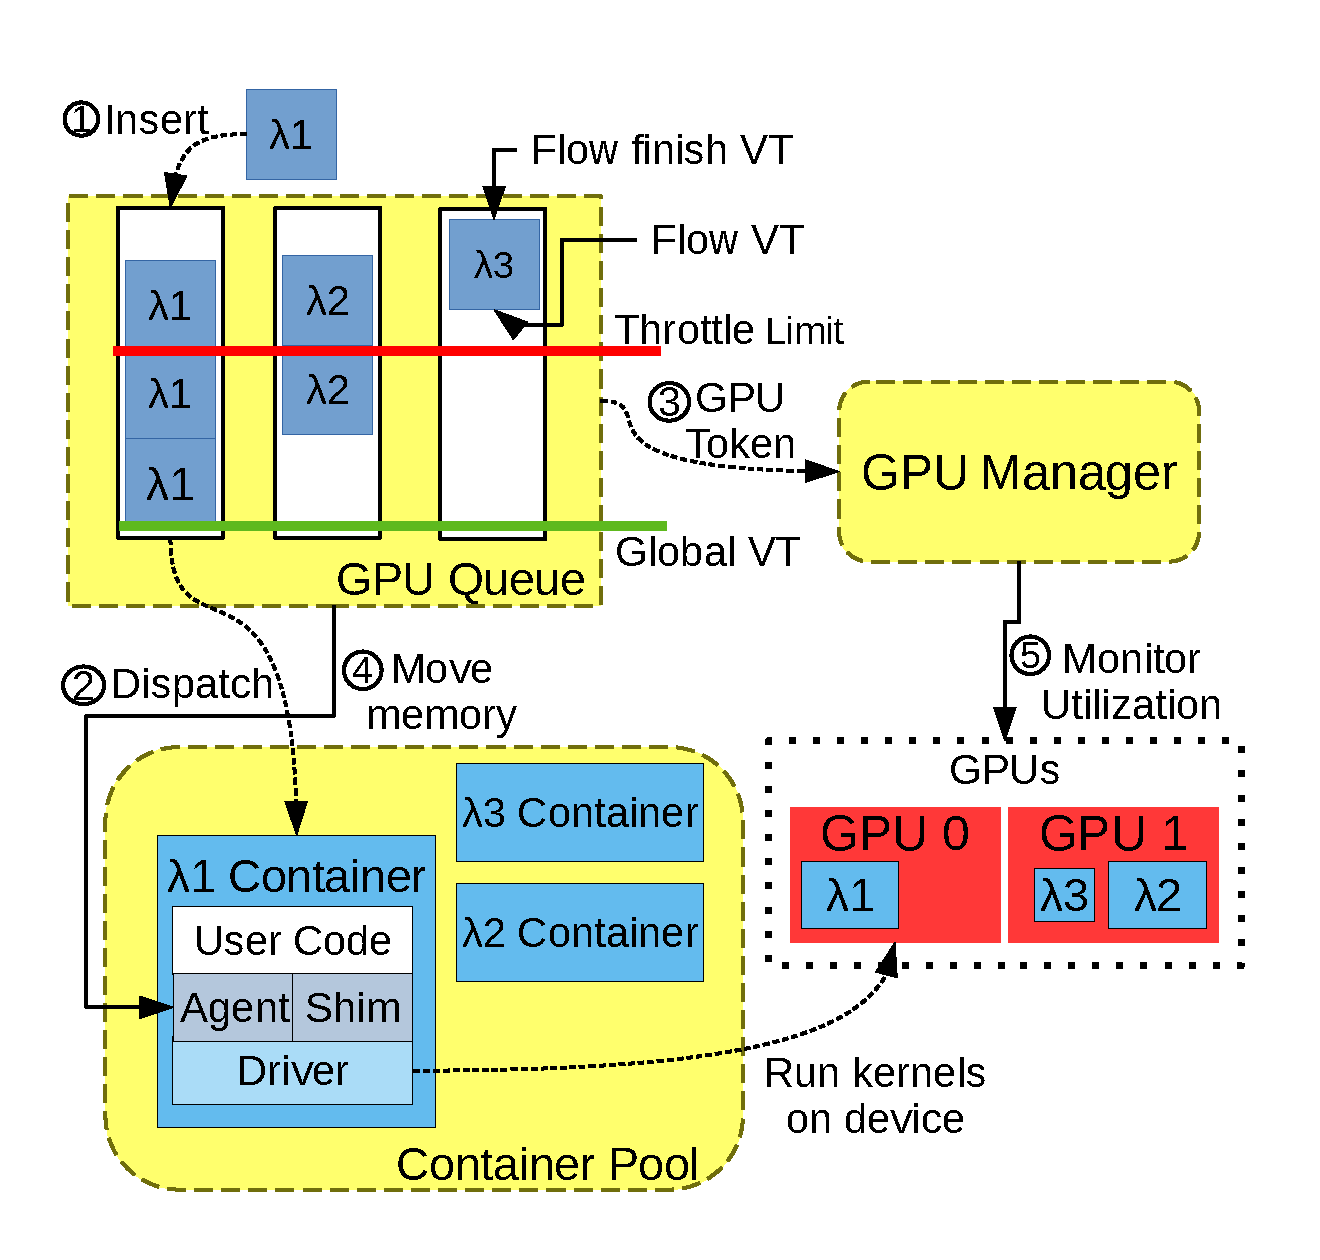
\includegraphics[width=0.8\textwidth]{./mqfq-final/figs/queue-sys-2-simple.pdf}
  \caption{Scheduling GPU functions as flows with Multi-Queue Fair Queuing. Invocations are dispatched based on the virtual time. The container pool helps with warm starts.}
  \label{fig:sys-diag}
  % \vspace{-0.6cm}
\end{figure}


\subsection{Key Insight: GPUs as Multi-Queue I/O Devices}
\label{sec:d:mqfq}

We claim that the tradeoffs and challenges of guaranteeing fairness and high throughput for serverless GPU workloads are similar to modern I/O scheduling.
Specifically, we can view GPUs as multi-queue I/O devices, and use fair scheduling algorithms like MQFQ~\cite{hedayati2019multi} to provide a rigorous and well-tested conceptual framework.
From a workload perspective, the I/O heterogeneity and fairness of different applications is similar to FaaS functions' heterogeneity.
Similarly, modern disks have multiple internal dispatch queues, which also maps to the temporal and spatial multiplexing offered by GPUs.
Successive invocations see lower latency from temporal and even spatial locality, a fact requiring significant attention when maximizing throughput.

Our scheduler maintains multiple dispatch queues, each queue corresponding to an individual function.
These queues (also called \emph{flows}) hold invocation requests which are analogous to disk read/write requests.
Multiple invocations dispatched from a single flow preserve temporal locality and benefit from warm starts.
The GPU, just like modern NVMe disks, also supports parallel dispatches, and we keep a subset of flows in the \quotes{active} state.
Flows without en-queued invocations are \quotes{inactive}.
Fair queuing uses the notion of virtual time (\VT) to capture the amount of service rendered to flows (normalized by priority weight).
The flow's \VT~grows by a fixed increment after an item is removed and dispatched for execution.
Flows are selected for dispatch based on their \VT's, and fairness arises from a bound on the maximum difference of flows \VT's.

Our insight is that the above classic fair queuing framework can be extended to meet the challenges of serverless GPU scheduling.
Locality is maintained by dispatching successive requests from an active flow, by borrowing ideas from anticipatory scheduling and using MQFQ's concurrent dispatch, which increases throughput but still maintains fairness (albeit with a larger inter-flow \VT~bound compared to classic fair queuing with a single active flow).
Each flow can be handled by a separate thread which can dispatch requests concurrently, taking advantage of device-level parallelism.
The amount of device parallelism is configured and controlled via tokens with the \D~parameter (Table~\ref{tab:mq-symbols}). 
To prevent popular functions from monopolizing the GPU, flows are \emph{throttled} if their \VT~exceeds the global \VT~(\GlobVT) (which is the minimum of all flows' \VT) by a certain threshold (\T).
\emph{Fair queuing provides the necessary parameters for principled and tunable batching in an online manner, for highly dynamic and heterogeneous FaaS workloads.}

\begin{table}
  \caption{Key symbols and parameters for \QName.}
  \label{tab:mq-symbols}
  \begin{tabular}{c|l}
    \hline
    Symbol & Description \\
    \hline
    \VT & Virtual Time, device wall clock service time accrued by a flow \\
    \GlobVT & Minimum \VT~across all active flows \\
    \T & Amount any flow's \VT~can exceed \GlobVT~before being throttled \\
    \D & Device concurrent invocations, can be fixed or dynamic with an upper-bound \\
    % \FinVT & A Flows \quotes{Finish}~\VT, the flow's \VT~plus its length by average execution time \\
    TTL & Time-to-live for an empty flow to become inactive \\
    % Service Average & Amount by which a flow's \VT~is increased after dispatch \\
  \end{tabular}
\end{table}

\subsection{MQFQ-Sticky: Locality-enhanced Fair Queuing}
\label{sec:mq}

% Want to enhance the locality of MQFQ.

The above MQFQ scheduling framework was designed for I/O.
However, GPU functions have different compute and memory footprints, execution runtimes, and cold vs. warm execution times; all of which diverge from disk assumptions. 
The GPU device model is also different: the device parallelism is lower (SSDs support hundreds of active threads), and execution performance is highly sensitive to utilization and interference. 
We therefore modify the original MQFQ design to account for these differences, to get the maximum performance out of our accelerators. 

% Tasks sent to sold-state disk I/O use equal amounts of device time and resources.
% Their GPU function counterparts can vary widely in both of these metrics, including between invocations of the same function.
% Disks can also handle over 100 parallel requests, and GPUs see execution overhead with single-digit concurrency that also is dependent on compute and memory usage.

Unlike disk requests with uniform block sizes, function execution times can vary significantly.
% This is a NOVELTY of ours, not in MQFQ. Also VT is not updated on insertion, that statement is wrong. You're thinking of the per-invocation VT / a flows Finish VT being incremented
% A new invocation is inserted into its function's flow, and the flow's \VT~is incremented based on the function's expected execution times. 
We account for this by tracking the historical average execution time $\tau_k$ of each function $k$, and when an item is dispatched, its flow's \VT~is instead incremented by $\tau_k/w_k$, where $w_k$ is the priority weight of the function.
Thus shorter functions are allowed more \emph{invocations} than their long counterparts, but both get equivalent wall time on the GPU.
% WRONG. Always updates to the GLOBAL MINIMUM across all flows. Updating like this causes serious divergence in global VT
% When an invocation is dispatched, the global \VT~is updated to the flow's \VT~as long as the \GlobVT~monotonically increases (i.e., $\GlobVT~= max(\GlobVT, flow.\VT)$). 
After an invocation is dispatched, \GlobVT~is updated if necessary to a potentially new global minima across flow VTs.
%(i.e. $\GlobVT~=~min(\forall flow.\VT~\in~Flows)$).

Since GPU memory is limited, we use the flow states for \textbf{proactive memory management.}
Flows that become active have their data moved onto the device in anticipation of use (if space is available). 
When a container is about to execute, we proactively move all its data to the GPU. 
Conversely, throttled and inactive flows have their data moved off-device, because we don't expect them to run in the near future. 
% Reclaiming device memory allows us to warm an active flow's data, data movement details are described in Section~\ref{sec:design-cont-shim}. 
More details about the data monitoring and movement are described in Section~\ref{sec:design-cont-shim}. 
Further modifications of ours pertain to how functions are drained and added to the queues, and are described below. 

\mhead{Anticipatory Scheduling}
Function performance is impacted by the availability of a warm container, and data in GPU memory.  
We introduce anticipatory scheduling to MQFQ to maximize the use of both. 
Anticipatory scheduling for disks~\cite{iyer2001anticipatory} boosts locality by keeping request streams \quotes{active} even if they are empty, in anticipation of future requests, which is especially beneficial for interactive applications.  
If a flow is empty (i.e., it has no pending invocations), then instead of immediately marking it inactive, we provide a grace period.
Without this grace period, because of the proactive memory management described above, functions would see their warm containers immediately removed from GPU memory.
%
Instead, we keep empty flows active for a configurable TTL (time to live), based on the function's inter-arrival-times.
Specifically, we set the flow TTL to $\alpha \times \text{IAT}$, where $\alpha$ is a tunable parameter. 
This policy is guided by the observation that reuse-distance is long-tailed~\cite{faascache-asplos21}, so a single global TTL is not ideal for both popular and rare functions. 

\mhead{Flow Over-run}
Our second technique for improving warm starts is to allow the flows to dispatch invocations in small \quotes{mini-batches}.
An active flow's start time is allowed to be \T~units ahead of \GlobVT.
\T~is the second main configurable parameter: larger values will result in larger batches and more locality, but less fairness, since functions will have to wait longer before their batches are dispatched.
If $flow.\VT + \T \ge \GlobVT$, then the flow is \emph{throttled}.
It may return to the \emph{active} state only after other flows get to run and the \GlobVT~increases. 


\mhead{Device Concurrency and Feedback}
% A device's concurrency limit \D~is not pre-determined as in the disk case.
% We must 
Because each function uses different amounts of compute and memory during execution, a fixed level of device parallelism (\D) like in disk scheduling may be sub-optimal.
We therefore track memory usage of running containers and GPU utilization to adjust \D~dynamically, to minimize contention and execution overhead.
This utilization-based feedback permits different scheduling rates based on the dynamic workload characteristics.
We take two input parameters: the device utilization threshold (such as 90\%), and the maximum parallelism level (irrespective of utilization).
A coarse-grained controller loop runs every 200 ms to check the real-time utilization and changes the \D~level dynamically to ensure the utilization is under the threshold.
Higher thresholds increase utilization and reduce queuing, but risk higher performance interference. 
% These methods are described in detail in Sections~\ref{sec:gpu-man} and~\ref{sec:design-cont-shim}.
More details of memory usage and GPU monitoring are described in Section~\ref{sec:design-cont-shim} and Section~\ref{sec:gpu-man} respectively. 

\mhead{Dispatch Concurrency}
In classic MQFQ, flows can concurrently dispatch their requests (as long as they are within the \T~threshold).
From a FaaS control plane perspective which needs to track invocation status carefully, we prefer a \emph{single} dispatch thread which picks the eligible candidate flow queue (such that $flow.\VT < \GlobVT + \T$).
Thus, the dispatch is not concurrent, which results in the most fair outcome via selecting flow with the lowest \VT~(i.e., earliest arrival).
However, this reduces locality and batching opportunities, resulting in poor function performance.

To remedy this, we pick the next flow from the set of candidate flows by sorting on both recency and locality, as shown in line~\ref{lst:line:filter} of Algorithm~\ref{algo:dispatch}.
Our heuristic prefers longer queues which provide more batching opportunities and reduces their larger backlog.
Ties are broken in favor of the flow with the least number of currently executing invocations (Line~\ref{lst:line:in_flight}).
This encourages multiple flows to progress and reduces the chance of a cold start caused by concurrent execution of the same function.
% In both cases we are draining the most backed up queues and enabling flow stickiness.
Flow stickiness from this heuristic provides sufficient temporal locality between active flows to maximize throughput.
This completes the description of the key attributes of our MQFQ-Sticky algorithm.
We note that it maintains the fairness properties, since we are basically emulating dispatch concurrency, but prioritizing longer flows within the eligible flow window.
That is, we still retain the MQFQ fairness property, which states that the service received ($S$) by two active flows during a span of wall-clock time $(t_1, t_2)$ is bounded by:

\begin{equation}
  \label{eq:fairness}
 \left|\dfrac{S_i}{w_i} - \dfrac{S_j}{w_j} \right| \leq (D-1) \left(2T + \dfrac{\tau_i}{w_i} -\dfrac{\tau_j}{w_j} \right)
\end{equation}

Because of the controlled concurrency, a smaller bound may be possible for \QName, which is part of our future work. 
The intuition is that classic MQFQ has $O(T!)$ possible permutations for dispatch, whereas our heuristic restricts the permutation space which is a strict subset. 

\algnewcommand{\LineComment}[1]{\State \(\triangleright\) #1}
% \begin{figure}
\begin{figure}[t]
\begin{algorithm}[H]
\caption{\QName~algorithm.}
\label{algo:dispatch}
\begin{algorithmic}[1]
\Procedure{Dispatch}{}
\State $\GlobVT \gets min_{f \in \text{flows}}(f.\VT)$
\State $chosen \gets None$
\For{$flow \in flows $}
\State $update\_state(flow, \GlobVT)$ \label{lst:line:update_vt} %\Comment {Set Inactive/Throttled}
% \If{$flow.is\_active() \textbf{ and } !flow.is\_empty()$}
%   \If{$chosen == None$}
%     \State $chosen \gets flow$
%   \ElsIf{$chosen.finish\_vt < flow.finish\_vt$}
%     \State $chosen \gets flow$
%   \EndIf
% \EndIf
\EndFor
% \State $to\_select \gets max(3, \D)$
% \State $sort(flows, on: \FinVT)$
% \State $flow\_cnt \gets max(0.3*num\_active\_flows, \D)$
% \State $candidates \gets top(flow\_cnt, flows)$
\State $cand \gets filter(flow.active \wedge flow.len > 0, flows)$ \label{lst:line:filter}
\State $sort(cand, on: length)$
% \State $chosen \gets max(candidates, on: length)$
\If{$\D \ne 1$}
\State $sort(cand, on: in\_flight)$ \label{lst:line:in_flight}
\EndIf
\State $chosen \gets top(cand)$
\State $token \gets get\_\D\_token(chosen)$
\If{$token == None$}
\State \Return $None$
\EndIf
% \State $mindicator.update\_vt(chosen)$
\State \Return $chosen.pop()$ \label{lst:line:done}
\EndProcedure
\\
\LineComment{Update state of flow, given the global \VT}
\Procedure{update\_state}{flow, \GlobVT} \label{lst:line:update_state}
\If{$flow.is\_empty~\textbf{and}~flow.in\_flight==0$}
\If{$Date.Now() - flow.last\_exec \ge TTL$}
\LineComment{Flow has expired}
\State $flow.state \gets Inactive$
\EndIf
\ElsIf{$flow.\VT - \GlobVT < \T$}
  \LineComment{Flow has exceeded threshold}
  \State $flow.state \gets Throttled$
\Else
\State $flow.state \gets Active$
\EndIf
\EndProcedure
\end{algorithmic}
\end{algorithm}
\end{figure}

\subsection{Integrated Memory Management and Scheduling}
\label{sec:design-cont-shim}


Each container has a custom shim that intercepts calls to the GPU driver, specifically those for initialization and memory allocations.
Requests by functions to allocate physical memory are captured in and converted into UVM (virtual device memory) allocations, allocation metadata is stored, and the result is returned to function.
We use MQFQ flow states to guide memory movement.
When some flow becomes active, all its CUDA-malloc'ed regions are \emph{prefetched} into the GPU memory, in anticipation for continued use.
We introduce and maintain a \emph{container pool} of such created GPU containers, and executions of the function results in a \emph{GPU-warm} start.
The efficacy of this container pool is restricted by physical GPU memory, and thus throttled and inactive flows have their regions marked for eviction.
This entails swapping and moving their GPU memory regions back to the much larger host CPU memory, with this eviction done asynchronously using LRU (least recently used) order.
In rare cases, a throttled and swapped out flow may get invoked again, which leads to a \emph{``GPU-cold but CPU-warm''} start since the container is already fully initialized, but data dependencies are not located on device. 
% , and the CPU container pool uses all the server DRAM which is several orders larger than GPU memory.
In the above case, prefetching may need to evict some other container's GPU regions, increasing latency. 

%the queue, via our agent inside each container, directs the shim to move the memory for the flow's containers onto the device in anticipation of use.
%In the event memory pressure is too high, this is delayed until an invocation is about to be dispatched, and only the container about to execute migrates memory.
%When a function's flow is inactive or throttled, we again use the shim to move container memory off the device to free up space.
%Because our shim tracks memory metadata, we can know how much memory a container needs on-device, and our GPU monitor ensures we don't over-subscribe memory with running invocations.
%Memory management implementation details and microbenchmarks are provided in the next section.
% Our driver can move the memory on and off the device to ensure

\subsection{Multi-GPU Load Management and Feedback}
\label{sec:gpu-man}

% System utilization feedback driven 

The GPU monitor is responsible for two key mechanisms: tracking GPU assignment and monitoring GPU utilization.
Creating a GPU context uses physical memory we can't control, so the monitor only allows a fixed number of containers to exist at one time.
Note that we support multi-GPU systems, and still maintain a single set of MQFQ flow queues per system.  
New functions are launched on the GPU with the most available resources and future invocations of the function run on the same GPU to take advantage of locality. 
%When is required but not available, we use this mapping to evict a container to make room.
% When a slot isn't available, we use this mapping to evict a container using an LRU caching strategy to get a slot on the device that we want to run on from Section~\ref{sec:design}.

Dynamically setting \D~is dependent on the two computing and memory resource limitations of GPUs. 
Because we intercept memory allocations, we can closely track device memory usage of containers thanks to our driver shim, and only allow a new dispatch when the needed container won't overload the device's physical memory. 
Ensuring there is available compute is not as straightforward to manage as memory due to unpredictable function characteristics.
An ML inference task for example could have known compute usage, since input and weight tensors have fixed uses based on the execution graph.
Other types of GPU functions can launch compute kernels unpredictably, based on the application's internal control flow.
The actual size and number of kernel launches often vary with function arguments, making an a priori utilization intractable.
Accepting this, we choose to externally monitor device utilization and launch new invocations when headroom is deemed sufficient to support another dispatch.
To avoid a thundering herd of launches, we increment the tracked usage by a factor of $1/\D$, and let the next monitoring update capture actual usage.
When both resources are deemed available for a dispatch, we \quotes{increase} \D~by allowing the item to start executing.
For this additive increase control-loop, we require $D_{\text{max}}$ as another parameter for providers to set upper-bounds based on the workload and service requirements.
%Our active management of both resources changes the nature of \D~from a fixed limit to controlled and usage-based concurrency. 
% Tracking both container/GPU mapping, and GPU utilization to allow function to start running

% \vspace*{\subsecspace}
% \subsection{Fairness Guarantee}

% \todo{Defend still fitting in MQFQ fairness theorem.}


%%% Local Variables:
%%% mode: latex
%%% TeX-master: "paper"
%%% End:


\section{Implementation}

We have implemented the keep-alive and the provisioning policies as part of our FaasCache framework built on top of OpenWhisk (Figure~\ref{fig:sys}). 

\begin{figure}[t]
  \centering
  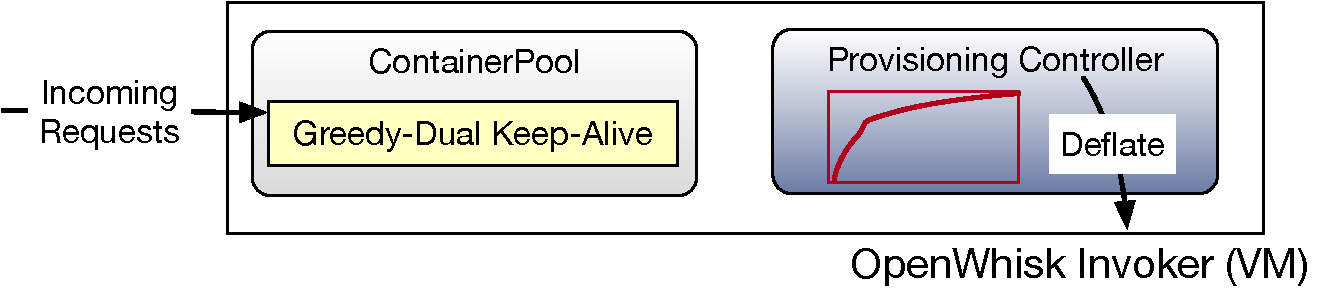
\includegraphics[width=0.95\textwidth]{faascache/faas-keepalive-20/figures/faascache.pdf}
  \caption{FaasCache system components. We build on OpenWhisk and augment it with new keep-alive policies and a provisioning controller. }
  \label{fig:sys}
\end{figure}

\noindent \textbf{Keep-Alive.}
FaasCache replaces the default OpenWhisk TTL-based keep-alive policy with the Greedy-Dual-Size-Frequency approach. 
For each initialized container, we assign and maintain the keep-alive prioritized ContainerPool, which is only a 100-line Scala modification. 
%Initialized containers are managed by the ContainerPool.
%\emph{Interesting aspects of priority calculation?} How is size, clock, frequency, cost, etc. computed? How does the impl differ from the idealized description? 
Each invocation of a function (OpenWhisk action) in ContainerPool records the launch time and when results are returned.


If the container was prewarmed before the invocation arrived, we record it as the function's warm runtime.
For new functions, the initialization overhead is captured and assumed to be the worst-case runtime until a warmed invocation is recorded. % is approximated as the minimum overhead of Docker and OpenWhisk's Python runtime initialization.
In the subsequent invocations, the initialization overhead is computed by subtracting the cold from the warm time. 
%Otherwise it was a cold start.
%The maximum cold and warm runtimes are kept per function to compute the priority.
%Size is simply the number of megabytes of memory OpenWhisk preallocates to the action's container, and
The function's frequency and clock value are updated with each request.
If the last container of a function is evicted, its cold and warm runtimes are stored and used to compute priority for its future invocations. 
%
To preserve the invocation fast-path, the ContainerPool is not kept sorted by priority. 
%Priorities are computed when an eviction needs to be made to reclaim memory.
Instead, it is sorted by priorities only during evictions, when the lowest priority container(s) are terminated.
%
We batch eviction operations to optimize the slow-path: we evict multiple containers to reach a certain free resource threshold (1000 MB is the current default). 

%rev 1
In the future, we intend to implement a similar design that is found in the Linux kernel page eviction. A separate thread (analogous to kswapd) can be used to periodically sort the containerpool list and asynchronously evict containers, so that eviction is not on the critical path. 

%All of an action's containers share one priority, regardless of the last time each ran an invocation.

% \prat{How are the values inferred?}
% New functions always replace old functions in the ContainerPool, so the priority of newly inserted containers doesn't matter. 
% After the second invocation of a function, its initialization overhead is inferred as the difference between the cold (first) and warm (subsequent) invocations. 
% Memory usage of the container is gathered via {\em Docker stats?\/}.



\noindent \textbf{Provisioning.}
For the static provisioning, we compute the reuse distance distribution for a given workload trace, and assume stationarity --- that it will be applicable on similar future workloads. 
We compute the reuse distances conventionally, by examining all reuse-sequences.
The dynamic provisioning controller runs periodically (every 10 minutes), to deflate or inflate the VM size, if the cold start rate deviates from the target significantly (by more than 30\%).
When the VM has to be shrunk, we use cascade deflation~\cite{deflation-eurosys19}.
We shrink the ContainerPool first, and reclaim the free memory using guest OS-level memory hot-unplug and hypervisor-level page swapping. 
%This approach is based on cascade deflation proposed in~\cite{deflation-eurosys19}. 

%Optimizations such as SHARDS that can significantly reduce the running time by sampling a small fraction of the functions, were found to be inadequate due to the wide disparity in the function sizes.
%The efficacy of sampling based techniques like SHARDS has mainly been empirically established only for fixed-sized objects. 


\noindent \textbf{Keep-alive Simulator.}
We have implemented a trace-driven discrete event simulator for implementing and validating different keep-alive policies.
Our simulator is written in Python in about 2,000 lines of code, and implements the various variants described in Section~\ref{subsec:variants}. 
It allows us to determine the cache hit ratios and the cold start overheads for different workloads and memory sizes.
Additionally, it also implements the static and dynamic provisioning policies for adjusting server size.

%%% Local Variables:
%%% mode: latex
%%% TeX-master: "paper"
%%% End:


\vspace*{-0.4cm}
\section{Experimental Evaluation}
\vspace*{\subsecspace}
\label{sec:eval}


Our experimental evaluation is examines the effectiveness of our scheduling based approach for opportunistic GPU acceleration for FaaS workloads for three main metrics: i) on-GPU execution latency (which captures how efficiently we are using the hardware), ii) per-function end-to-end latency which includes the queue wait time, and iii) device utilization and throughput for hybrid CPU-GPU systems.


% Run on system with Ubuntu, 48 phys cores, Nvidia P100 GPU, 250 Gb ram
% Here we will showcase the effectiveness of our GPU memory manipulation in minimizing

\mhead{Setup and Workloads}
All experiments were run on servers running Ubuntu 20.04 on kernel version 5.4, with a 48 physical core Intel Xeon Platinum 8160 CPU with hyperthreading disabled, 250 GB of RAM, and an Nvidia V100 GPU running driver version 470.239.06. 
This isn't the latest GPU hardware, and emphasizes that our design can work with a variety of hardware, doesn't require advanced features, and is easily scalable and adaptable to other systems.


Function were sampled from Azure trace~\cite{shahrad2020serverless} in the same manner as previous works~\cite{fuerst2023iluvatar,faaslb-hpdc22}, and function frequencies are scaled using the empirical CDF of the inter arrival times, to yield workload traces of different intensities.
Based on the execution times, we select the closest matching GPU function from Table~\ref{tab:gpu-cpu} that doesn't exceed that time. 
Each experiment is run with the same trace composed of 24 functions, run for 10 minutes, and presented results are the average of 5 repeated runs.
We evaluate on multiple traces with different function mix and invocation frequency distribution, providing a wide spectrum of realistic workloads with different heterogeneity and device loads (Table~\ref{tab:scaling}).
Although \QName~is capable of enforcing per-function QoS, we set the weight of all functions to 1, for ease of exposition. 
The evaluation is presented in a top-down manner: we first analyze the end-to-end latency, then show scaling behavior, and finally investigate the effect of various \QName~parameters described earlier in Table~\ref{tab:mq-symbols}. 


% \mhead{Crossplatform verifcation on Jetson} 
% To verify correctness of our implementation across platforms, we tested it on Jetson AGX Orin, a popular edge device with an integrated Ampere Architecture GPU \cite{jetson-specs}.
% We ported GPU functions cupy, onnx-roberta, tf\_imagenet and tf\_squeezenet by rebuilding them with 
% Machine Learning Container for Jetson and JetPack (l4t-ml:r35.2.1-py3) \cite{l4tcontainer}. 
% Jetson environment had Ubuntu 20.04, L4T version 35.4.1 and JetPack version 5.1.2 setup on it with 
% driver versions 11.4.315 for CUDA, 8.6.0.166 for cuDNN and 8.5.2.2 for TensorRT.
% On tegra platforms iGPU (integrated GPU) use system memory, therefore it's not possible to overcommit and for a dGPU (discrete GPU) unified memory is not supported currently \cite{tegra-uvm}. 
% Our shim is able to intercept and replace allocation calls but it does not have any impact. 
% Therfore, our implementation works without being able to overcommit on Jetson Orin AGX.

\mhead{Scheduling Policies}
To examine the locality, fairness, and utilization tradeoff, we implement and evaluate three \emph{additional} scheduling policies in addition to our default \QName. 
% \naive~dispatches function invocations in a first-come-first-serve order and has no container pool, and represents the umoptimized baseline for black-box GPU functions. 
The second policy is \fcfs, which uses the warm pool and memory management (we move function memory on-device before executing, and move it back off after each invocation has completed).
This represents a scheduling policy with most of the important GPU optimizations, but one which is not fully locality or fairness aware.
Our third and final scheduling policy variant is \batch, which also uses all the GPU optimizations, and maximizes locality by batching invocations of each function individually.
Unlike \QName, \batch~greedily maximizes batch sizes (and hence locality) irrespective of the build-up of other functions.  
% and a \texttt{Batch} policy that separates flows and executes everything in the flow with the

Using the MQFQ design allows for easy parametrization and implementation of these and other policies for exploring the locality vs. performance tradeoff.
Both \fcfs~and \batch~use the integrated memory management and CUDA interposition shim, and thus allow us to separate out the impact of \QName's core ideas with minimal code changes and differences. 
For \fcfs, all functions are inserted into a single queue.
For \batch, we insert invocations into per-function flows, and dispatch the entire \emph{flow} containing the oldest item. % to execute all removed items serially, but prevents new items from tagging along.

%\vspace*{-0.5cm}
\subsection{GPU Scheduling Performance}
\label{sec:queue-perf}

\begin{figure*}
  \centering 
  \subfloat[\textbf{Average latency} is significantly lower with \QName~for different device-parallelism (\D) levels.  \label{fig:queue-e2e}]
  {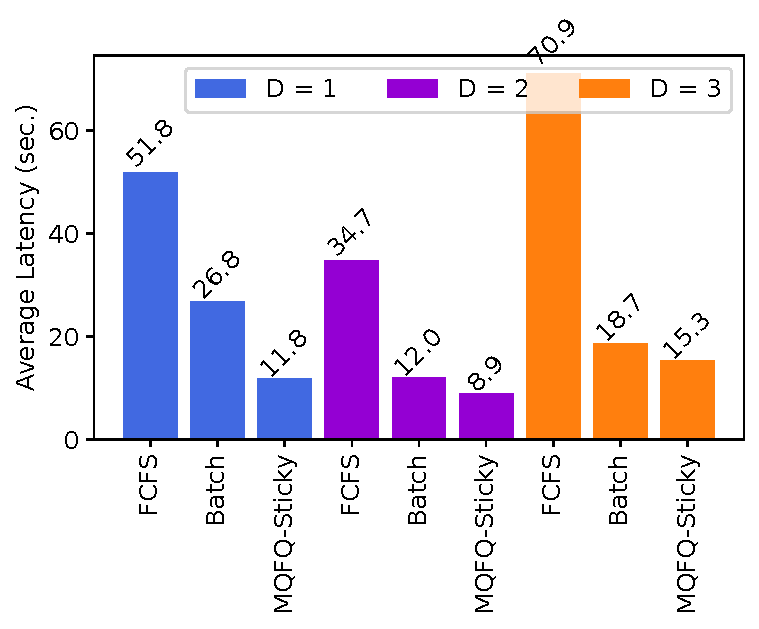
\includegraphics[width=0.32\textwidth]{../graphs/q_compare/25.7095/20/no_naive_e2e_sec.pdf}}
 \hfill  
\subfloat[The average and variance of \textbf{per-function latency} is much lower with \QName.  \label{fig:queue-fairness}]
{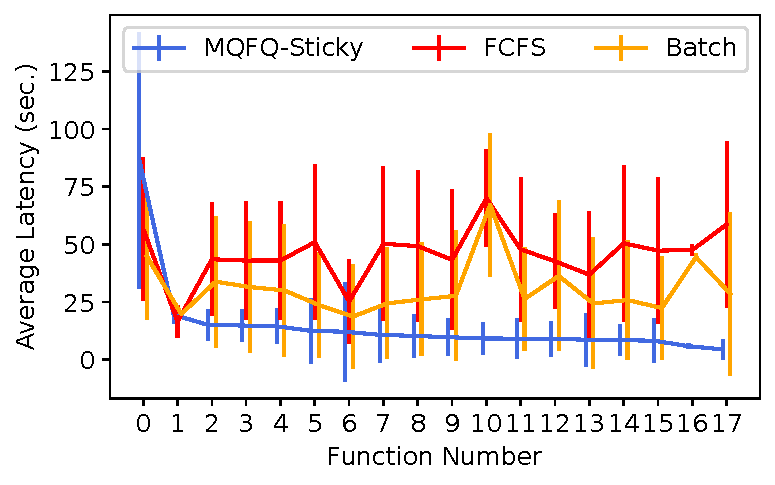
\includegraphics[width=0.35\textwidth]{../graphs/q_compare/25.7095/20/paper_fairness.pdf}}
\hfill 
\subfloat[\textbf{Device utilization} for the medium-load trace. \label{fig:util} ]
{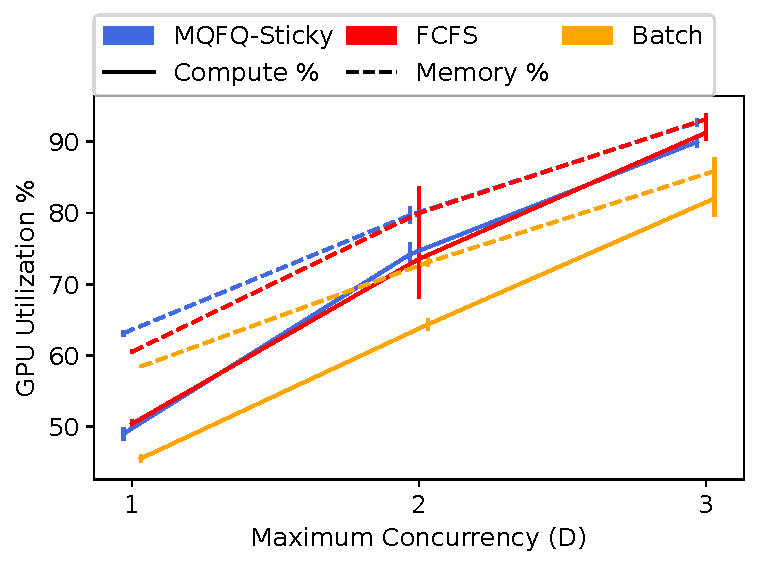
\includegraphics[width=0.3\textwidth]{../graphs/q_compare/25.7095/20/all_util_no_zeroes.pdf}}
\label{fig:base-all}
\vspace*{-7pt}
\caption{Latency, fairness, and utilization for a medium-intensity FaaS workload.}
  \vspace{\myfigspace}
% average variance across functions:
% 25.708
% mqfq,fcfs,batch
% 306.3366558710925 1775.2016313919078 1541.5163353200303
%
% 25.7095
% mqfq,fcfs,batch
% 260.76811271061183 752.4597314354334 664.7010323038504
%
% 25.707
% mqfq,fcfs,batch
% 176.98634136793837 902.0644451782704 669.7400253032657
\end{figure*}

To characterize the differences in the above scheduling policies, we first show the empirical evaluation with a \emph{medium-intensity} workload, which comprises of 24 functions with an average arrival rate of 2 invocations per second. 
This workload results in average GPU utilization of around 70\% (Figure~\ref{fig:util}), and represents the average case. 

\noindent \textbf{Average Latency.}
The latency across all invocations is shown in Figure~\ref{fig:queue-e2e}.
Not shown in the figure is the current baseline \naive~scheduling with Nvidia-docker, which does not have a container pool and suffers from excessive cold-starts.
\textbf{The \naive~average latency is close to 3,000 seconds---a $300\times$ overhead.}
The high latency is because of every invocation results in a cold-start, causing a large queue buildup.
Note that our workload trace is open-loop, and thus invocations are generated at fixed intervals.


% \naive~has extreme wait times due to cold starts caused by the lack of warm pool. 
%as we saw in Fig.~\ref{fig:container-pool-cold-hits}.
% Adding the pool and memory management in \fcfs~gives over two orders of magnitude improvement in latency, even when only a single invocation is dispatched to the GPU (D=1 case).
\QName~outperforms \fcfs~by $5\times$ with a 11.8 vs 51.8-second average respective latency thanks to its locality and fairness oriented design.
\batch~has middle of the road performance, lacking fairness and advanced locality policies.
% , and 20\% better than \batch~because it doesn't throttle functions that hog GPU time well.
% Increasing the device concurrency (\D) improves \QName~latency by a further 15\%.
For this workload, at higher concurrency levels, \QName~improves latency by an additional 25\% to an 8.9-second average per invocation.
Both competing policies also benefit from concurrency, but neither outperform \QName.
% This is caused by errant lucky items at the end of batches jumping ahead in the queue, in violation of fairness principles.
When \D~is set too high (\D=3), the device cannot handle the higher concurrency, and all policies suffer varying degrees of degradation due to resource contention and interference.
For this workload, the queuing delays account for more than 99\% of the end to end function latency, and thus scheduling policies have significant impact. 
% Execution time is equal between all three policies, as they share the GPU monitor, latency improvements come entirely from more optimal scheduling decisions and reduced cold starts.
% \todo{Add queuing vs execution split for the latency results?}

\noindent \textbf{Fairness.}
In Figure~\ref{fig:queue-fairness}, we show the per-function latency (averaged across all its invocations).
We use inter-function latency variance as our fairness metric.
\fcfs~has the worst global inter-function latency variance (752), and the highest average latency.
\QName~reduces latency in the range of $2-10\times$, and has only one-third the inter-function latency variance of \fcfs.
Also, the invocation latency variance for each function (the error bars) is $3-4\times$ lower compared with \fcfs~and \batch.

\textbf{Result:} \emph{\QName~policy provides a $5\times$ reduction in average latency across all functions, and also reduces their jitter and tail latency by $3-4\times$.}

\vspace*{\subsecspace}
\subsection{Scaling}

We now look at load, GPU, and memory scaling properties of \QName.

\begin{table}
  \caption{The latency benefit of \QName~improves with increasing GPU utilization.}
  \vspace{\captionspace}
  \label{tab:scaling}
  \begin{tabular}{rrrrr}
    GPU Util (\%) & Req/s & \QName(s) & FCFS(s) & Batch(s)\\
    \hline
    28.025 & 1.122 & 3.932 & 7.843 & 4.962\\
    35.747 & 1.797 & 2.432 & 4.511 & 2.838\\
    38.889 & 1.943 & 3.434 & 8.031 & 3.441\\
    42.740 & 1.690 & 1.046 & 1.371 & 1.054\\
    43.347 & 2.572 & 2.929 & 7.309 & 3.454\\
    52.054 & 1.125 & 2.956 & 3.512 & 2.415\\
    57.467 & 4.263 & 5.630 & 37.743 & 9.585\\
    68.141 & 2.693 & 10.543 & 44.450 & 13.570\\
    74.216 & 2.553 & 8.899 & 34.719 & 11.996\\
  \end{tabular}
  \vspace{-0.4cm}
\end{table}

\mhead{Latency vs. load}
Table~\ref{tab:scaling} shows the latency for different workload traces, each with a different mix of functions and IATs (inter arrival times), resulting in different average GPU utilization.
In general \QName~performs better at higher utilization, reducing average latency by $4-6\times$ vs. \fcfs.
When considering the latency weighted by the number of invocations, and normalized to the no-interference case, the performance gap is even higher, since smaller functions are more affected by cold-starts and unfairness in relative terms.
\QName's weighted normalized latency is more than $10\times$ lower (vs \fcfs) at higher loads, and $2.5\times$ lower vs. \batch. 


\begin{figure}
  \centering  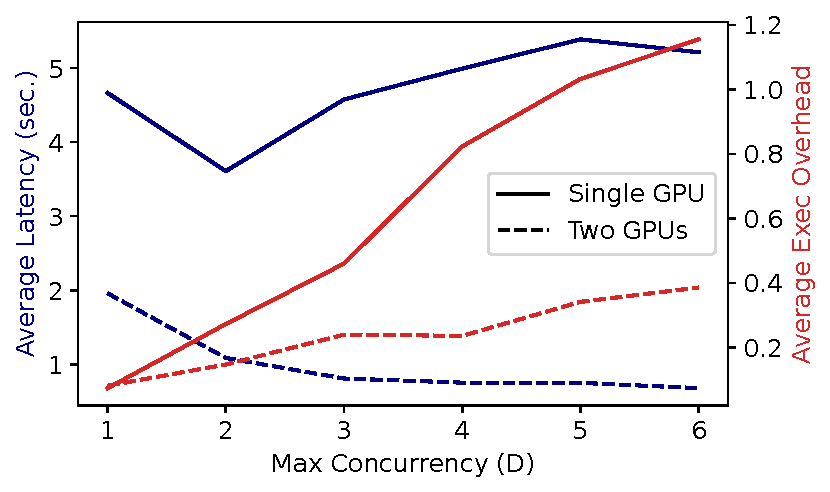
\includegraphics[width=0.35\textwidth]{../graphs/multi-gpu/25.7/concurr_scale.pdf}
  \vspace*{-8pt}
  \caption{\QName~also uses locality-aware scheduling for multiple GPUs, significantly reducing queuing.}
  \label{fig:multi-gpu}
  \vspace*{-8pt}
\end{figure}

\mhead{Multiple GPUs}
Our system easily scales to orchestrating and dispatching across multiple GPUs.
We run a high-load trace and show the comparison in Figure~\ref{fig:multi-gpu} after we add a second, identical, GPU to the server. 
% In Figure~\ref{fig:multi-gpu} we show how it adapts to running the same trace on systems with one and two identical GPUs.
Two GPUs not only allows us to run $\D\times2$ invocations, but also do on-the-fly load balancing between them to avoid compute contention with higher \D. 
% and therefore expect a corresponding 2x performance improvement.
As a baseline, the multi-GPU blue dashed line has $2.3\times$ lower latency at \D=1.
At higher device parallelism, the multi-GPU case sees a latency reduction of $4\times$ vs. the single GPU setting. 
Device parallelism also slightly increases the execution overhead due to interference, but is offset by the smaller queues. 

% Scaling \D~to 6, we see reductions in latency up to \emph{87\%} -- whereas the single device is quickly overloaded and has worse overall performance.
% % This balancing boosts latency reduction to \emph{87\%} when \D~is very high
% % , much better than our expected linear speedup.
% Execution overhead in red increases dramatically with \D~when only one GPU is available, in the worst case a nearly 6x increase.
% % With higher \D, our dispatches also load balance between the two devices, something not possible in the solitary device case.
% However, with two GPUs in the red dashed line, once $\D \ge 2$ the load balancing mitigation lowers overhead by 45\%, and a maximum of 66\%.
% Reduction of this overhead is a significant contributor to lower latencies as well.
% The ability to choose devices results in a 70\% reduction in execution overhead, entirely from mitigating compute overloading.



% e2e
% [4.663137860034904, 3.607658436985101, 4.575037657122783, 4.991578333097969, 5.386245616200919, 5.212470496279234]
% [1.9581354786418401, 1.0854709685368538, 0.8082406824696803, 0.7523517956355057, 0.7496512471943295, 0.677325266114725]
% [0.58008201 0.69912036 0.82333682 0.84927577 0.86082119 0.87005677]
% exec
% [0.07375773205618323, 0.27254631424617926, 0.4598690614061698, 0.8230379144178025, 1.0323527250435014, 1.154964442968281]
% [0.08146243318283061, 0.14722147302861147, 0.2398143374961277, 0.2358641959639591, 0.341338564858076, 0.3858309500976596]
% [-0.10445957  0.45982952  0.47851604  0.71342244  0.66935859  0.66593695]


\begin{table}
  \centering
  \caption{Hybrid CPU+GPU reduces latency by more than 2x compared to CPU-only and GPU-only execution.}
  \vspace{\captionspace}
  \label{tab:cpu-gpu}
  \begin{tabular}{|l|r|}
  \hline
  Case & Avg. latency (s) \\ \hline
  CPU-only & 2.03 \\
  1 GPU & 3.43 \\
  2 GPUs & 1.08 \\
  CPU+GPU & 1.00 \\
  \hline 
\end{tabular}
\vspace{-0.4cm}
\end{table}

\mhead{Hybrid CPU+GPU execution}
For evaluating hybrid execution, we use a GPU-speedup based dispatch policy.
We use offline profiling to obtain the GPU speedup for functions, and only run the top 50 percentile of functions on GPU, and rest use the CPU.
This corresponds to functions having GPU speedup of $>3\times$ being eligible for GPU acceleration. 
Other functions avoid queuing for the GPU and run immediately on the system's plentiful 48 CPU cores. 
The average function latencies are shown in Table~\ref{tab:cpu-gpu} for a high-intensity workload. 
Due to excessive queuing and contention, a single GPU degrades latency by 38\%. Adding a second GPU alleviates this load and reduces latency by half.
Interestingly, hybrid execution with the CPU and single GPU reduces latency even further, thus showing the benefits of heterogeneous hardware for FaaS workloads. 

% CPU 2.030147525728988
% GPU 3.4336443728988
% Two GPUs 1.0899518145507185
% CPU/GPU 0.9972267068610635


\begin{figure}
  \centering  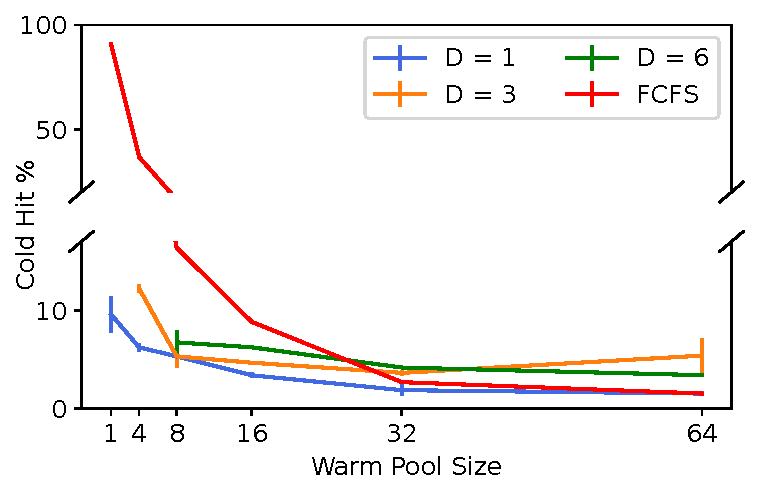
\includegraphics[width=0.30\textwidth]{../graphs/container_pool/big-60min/65/cold_hits.pdf}
  \vspace*{-8pt}
  \caption{Container-pool reduces cold-starts. \QName~provides higher locality.}
  \vspace*{-14pt}
  \label{fig:caching}
\end{figure}

\mhead{Container Pool Size}
% Functions running warm is vital for low latency in serverless systems which, and our UVM shim enables maintaining a warm pool of GPU containers.
For temporal locality, the invocation patterns and batching plays a key role in reducing cold starts.
The performance difference between \QName~and \fcfs~can be largely attributed to the cold-hit ratio of the invocations.
Figure~\ref{fig:caching} shows the \quotes{miss-rate curves} for the medium-intensity trace as we increase the number of containers in our container pool.
We focus on the number of containers in the pool, rather than MB of pool memory for simplicity.
Idle containers do take up CPU memory, and work managing the memory used by caching containers is orthogonal to our design~\cite{faascache-asplos21}.
Since \QName~prefers smaller batches of functions and does anticipatory keep-alive, it has a high temporal locality and its cold-hit \% is in the range of 2-8\% across a range of pool sizes and device concurrency.
In contrast, \fcfs~has 50\% cold-starts with a pool size of 4, and achieves parity with \QName~only at largest pool sizes when the popular functions can fit in the container cache.


\vspace*{\subsecspace}
\subsection{Impact of Scheduling Parameters}
\label{sec:queue-knobs}

In this subsection, we explore the effects of configuration knobs to see their effect on performance, which also sheds a light on the empirical relationships between fundamental parameters of locality and throughput. 


% \begin{figure}
%   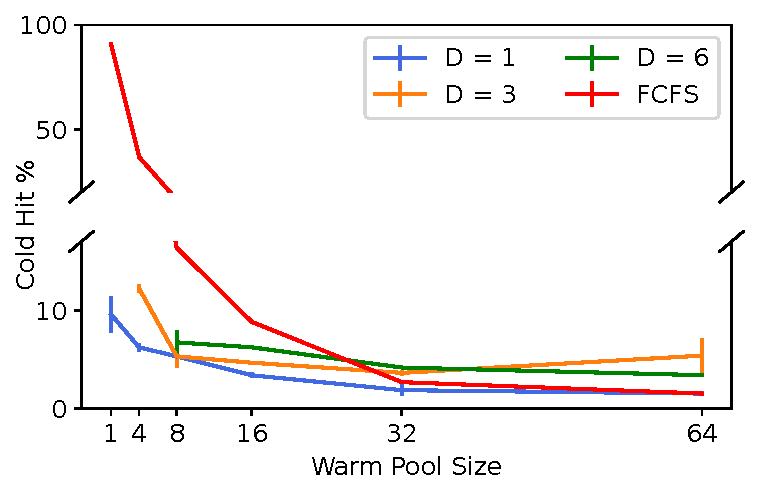
\includegraphics[width=0.4\textwidth]{../graphs/container_pool/big-60min/65/cold_hits.pdf}
%   \vspace*{\captionspace}
%   \caption{\QName~greatly reduces cold hits compared to FCFS, and is improved with a large container pool size. 
%           More cold hits are also caused when \D~(concurrency) is raised, needing private containers to serve concurrent invocations.}
%     \label{fig:container-pool-cold-hits}
%     \vspace{-0.4cm}
% \end{figure}

\begin{figure}
  \centering
  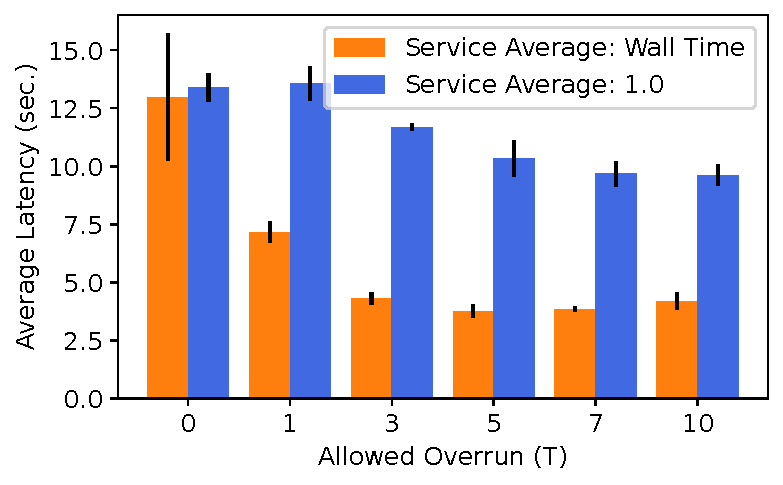
\includegraphics[width=0.3\textwidth]{../graphs/unfairness/25.7/e2e_sec.pdf} 
  \vspace*{-5pt}
  \caption{Larger T yields more batching and lower latencies because it allows popular flows to run ahead. Using historical function execution latencies helps significantly compared to uniform flow costs in classical fair queuing.}
  \label{fig:T-service}
    \vspace*{-7pt}
\end{figure}

\mhead{Flow over-run (\T)}
Recall that flow virtual times are within \T~of each other.
Larger \T~results in more locality and batching opportunities, but decrease fairness, since flows may get to monopolize resources for longer before being throttled.
Figure~\ref{fig:T-service} shows the average latency decreasing, but with diminishing returns, as the over-run is increased. 
The figure also shows the value of using function wall clock execution times.
When all flow usages are assumed to be constant (1.0 in the figure), long functions may dominate, which increases average latency by more than 3x.
\emph{Thus, a small amount of over-run guided by function characteristics helps significantly.}

\begin{figure*}
  \centering
  \subfloat[Anticipatory flow keep-alive (non-zero flow TTL) can reduce latency by up to 50\%. We use function IAT for scaling the TTL. \label{fig:flow-ttl}]
  {  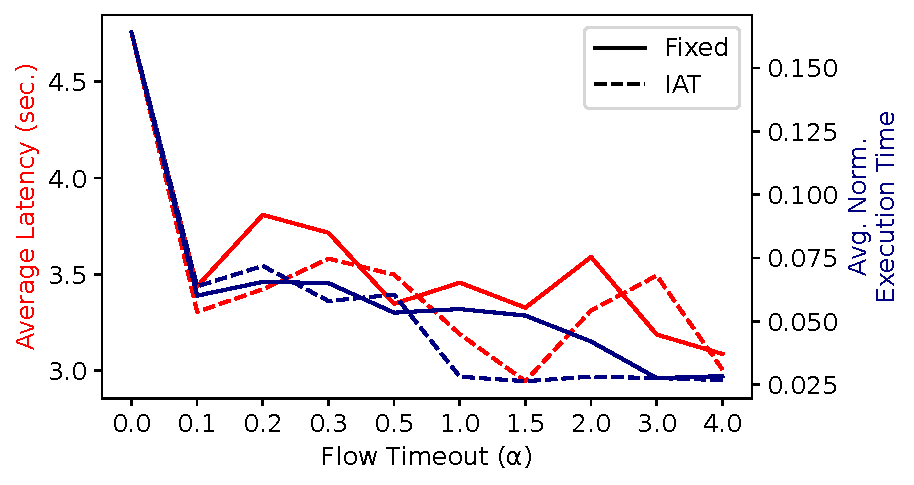
\includegraphics[width=0.35\textwidth]{../graphs/ttl/25.8/mqfq-ttl-compare.pdf}}
  \hfill
  \subfloat[Concurrent function invocations (\D) increase execution time due to contention. GPU utilization thresholds reduce overload. \label{fig:concur-exec-overhead}]
  {  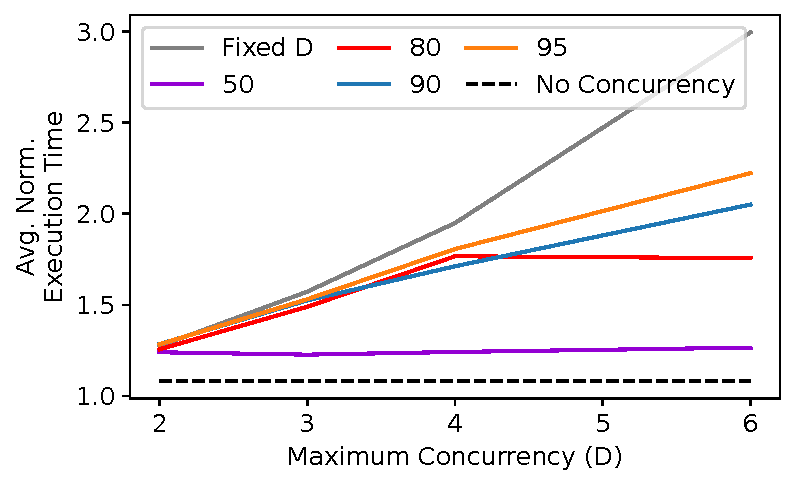
\includegraphics[width=0.3\textwidth]{../graphs/concurrency/25.7/paper_exec_overhead.pdf}}
  \hfill 
  \subfloat[Concurrent execution can reduce latency by reducing queuing. However, this is negated by execution interference  at higher levels.  \label{fig:concur-e2e}]
  {  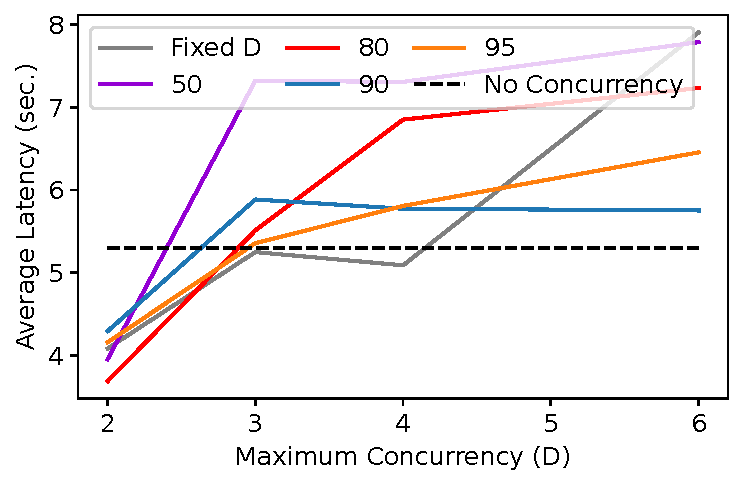
\includegraphics[width=0.3\textwidth]{../graphs/concurrency/25.7/paper_e2e_sec.pdf}}
  \vspace{\captionspace}
  \caption{Flow TTL and device parallelism (\D) are set based on workload and utilization.}
  \vspace{\captionspace}
  \label{fig:knobs-all}
\end{figure*}


\mhead{Flow keep-alive TTL}
Empty flows remain active until a TTL expires, after which they're made inactive and have their resources evicted.
Figure~\ref{fig:flow-ttl} shows the improvement to both execution time as compared to ideal warm performance and latency as the TTL grows.
The execution overhead is reduced because of warm start locality, and is the main factor behind latency reduction. 
Setting any global TTL (the solid line), at even a small 0.1 seconds, improves latency and overhead by 25\% and 50\% respectively. 
% Latency sees a 25\% improvement and execution time over 50\%, from \emph{any} TTL policy, and 
Increasing the TTL to up to 4 seconds sees significant, but diminishing, returns.


%For the \texttt{Fixed} line, the X axis represents time in seconds for the global TTL.
%For the \texttt{IAT} line, the X axis represents the factor by which each function's IAT was scaled to become its TTL.

% A large 4 second time can reduce latency by 35\% and execution time by 40\%.

By default, we base TTL on each function's inter-arrival-time (IAT), rather than have a global fixed time.
This method sets the TTL for each flow to the IAT multiplied by the value ($\alpha$) on the X axis, plotted as the dashed line.
For flow timeout ($\alpha$), our default range is between 1 and 2, which contains the minima, as shown for this particular trace (at 1.5).
Higher TTLs ($\alpha > 3$) may result in too many active functions and pressure on the container pool. However, our design is robust to very large TTLs: the pool uses LRU eviction and the resulting impact on performance even at high TTLs is low.
\emph{Thus, anticipatory scheduling improves latency by 50\%, and \QName~performance is not sensitive to the TTL.} 


\mhead{Device Concurrency}
We now explore the tradeoff due to device concurrency, which can improve utilization, but also risks performance interference and is dependent on the co-located applications, which are constantly changing in FaaS workloads. 
We run our medium workload and adjust device concurrency using \D~and examine the effect on execution time (without considering queuing delays) in Figure~\ref{fig:concur-exec-overhead}. 
% Figure~\ref{fig:concur-exec-overhead} examines the effect on execution overhead as the concurrency \D~is changed and is made dynamic.
All numbers are normalized to the no concurrency (i.e. $\D=1$) case. 
When we increase \D~and use a fixed value, shown in the gray line, we always have \D~number of invocations trying to execute on the GPU concurrently.
Normalized execution time is unsurprisingly correlated with \D, as GPU contention between invocations causes up to 100\% overhead at the maximum $\D=6$.


By default, we use the GPU utilization upper bound (shown by different lines in Figure\ref{fig:concur-exec-overhead}).
Setting the upper bound to 50\% utilization prevents over-saturation of the GPU, and reduces overheads significantly. 
However, this increases the queuing and total latency, as shown in Figure~\ref{fig:concur-e2e}.
For this workload, the total latency increases slightly due to contention and interference, and the limited memory of our GPU (16 GB).
The ``sweet spot'' is $\D==2$, and latency increases slightly by 30\% at higher levels.
Our present design leaves the maximum \D~to the operator, since the utilization based capping dampens its effect. 
\emph{Thus, allowing concurrent dispatch to the GPU, controlled to minimize contention, significantly improves global latency and utilization of the device.}

\textbf{Result:} \emph{Our introduced features such as flow over-run, anticipatory scheduling, utilization-driven concurrency, all contribute to latency reduction by $1.5-3\times$. A wide range of these parameters yield similar performance, making our system robust, yet still providing operators enough flexibility for fine-tuning based on workloads and operational requirements.}

\begin{comment}
% The remaining lines represent the GPU utilization percentage at which we dynamically adjust \D~but have a fixed maximum (\Dmax), represented by the X axis value.
In the remaining lines when we adjusted \D~dynamically with utilization as described in Section~\ref{sec:mq}, at varying thresholds.
For example the purple line limits \D~at 50\% utilization, and given this low number, does not see an increase in execution time because it refuses to dispatch, despite a growing maximum \D.
% The other utilization points allow more concurrent dispatches, and see increased execution times.
The 80\% line has a minor 1.2x normalized execution time, equal to that of 50\%, but reaches a higher plateaus with large \D.
Next we show the effect controlling \D~has on latency.
% all are more limited
% In the dynamic case, when the compute utilization is below 95\%, we increase \D~and dispatch a new invocation.
% \D~is capped by a maximum configuration setting to prevent runaway dispatching that can occur during time in between active function's kernel launches.
% All see a small increase in overhead when $\Dmax==2$, equal between all values.
% A low percentage such as 50\% has stable overhead close to that of when $\D==1$, but at the expense of high queuing time due to lack of dispatches.
% Higher \Dmax~sees them separate but reach a plateau of maximum overhead, as the GPU manager limits \D~as it detects high device contention.

% Execution time isn't the only metric impacted, 
% Latency for invocations is affected by \D, throughput at the expense of individual invocation execution time.
Latency in Figure~\ref{fig:concur-e2e} changes with \D, throughput at the expense of individual invocation execution time.
Both fixed and dynamic methods have roughly 20\% better latency than when concurrency is disabled, with our 80\% line improving by 30\%.
The minor increase in execution time from concurrency at this point is outweighed by throughput gains.
Setting \D~too large eliminates this gain by offsetting it with the high execution time overheads we saw previously, or long waiting periods for usage to reduce, shown in the 50\% line case.
% is decreased across the board when $\Dmax==2$, and nearly 20\% better than baseline when utilization monitoring is at 80\%.
These are similar to the results in Fig.~\ref{fig:queue-e2e} which used a different trace, showing that the effect of \D~can vary with the function makeup of load.
Allowing concurrent dispatch to the GPU, controlled to minimize contention, significantly improves global latency and utilization of the device.
% This trend does not continue, caused by queuing at the conservative level of 50\% and encroaching execution overhead at higher levels.
% The scalability of \D~hinges on a variety of factors: function workload composition, device compute capability, and device memory size.
% Larger devices can support more functions, but this can be offset by an equally expensive function to run.

\end{comment}

% There is nothing wrong with the graph. Fixed D is only better than the dynamic options at D==3 and D==4 for latency
% It has worse execution overhead at all these points.
% It also has worse latency at _all_ points D>2 than having NO concurrency (the dashed line)
% \{Investigate/fix the avg latency vs. D graph. Fixed D does best? Maybe keeping the exec overhead graph will suffice.}


%%% Local Variables:
%%% mode: latex
%%% TeX-master: "paper"
%%% End:


%\section{Discussion}
\label{sec:disc}

In this section, we reflect on how our ideas fit into the broader serverless computing ecosystem. 

\paragraph{Impact on colocated applications.}
The short execution lifecycles of serverless functions makes them a good workload to colocate with other long-running containers, VMs, batch-jobs, etc.
Such workload management architectures result in an additional layer of performance tradeoffs: the keep-alive policies not only influence function performance, but also the performance of other colocated applications.
Our provisioning policies in Section~\ref{sec:provision} can be used to find the appropriate keep-alive cache size based on the performance vs. memory-consumption tradeoff captured in the hit-rate curves.
Ultimately, the tradeoff between function and other colocated application performance is determined by their utility and revenue for the cloud provider. 
Nevertheless, our provisioning policies can provide a principled way to examine these tradeoffs, and is part of our future work.
 

\paragraph{Cluster-level analysis.}
Cluster-level function load-balancing and scheduling also affects keep-alive. 
Load-balancing policies determine the function load and distribution of function characteristics on servers. 
The function workload characteristics have a major influence on performance, as we have extensively discussed in Section~\ref{sec:eval} (e.g., Figure~\ref{fig:exec-overheads-all}). 
For instance, a stateful load-balancing policy which runs a function on the same subset of servers will result in better temporal locality, which in turn improves keep-alive effectiveness.
On the other hand, randomized load-balancing is simpler to implement and scale, but offers worse temporal locality to individual servers. 
We have deliberately focused our techniques and evaluation on a single-server setting, in order to provide modular and easily reproducible policies. 


\paragraph{Explicit initialization.}
There are many techniques for reducing the initialization cost, which can be combined with our policies. 
The cold start overhead can also be addressed by \emph{explicit initialization} of functions, in which the initialization code is provided as a separate, explicit call-back. 
For instance, OpenWhisk supports an \texttt{init} call into the function runtime, which can be executed before the function is triggered with the \texttt{run} call. 
%, which we described in Section~\ref{sec:tradeoffs}. 
This explicit initialization allows functions to be pre-warmed, and can be used to reduce the cold start overhead.  
However, explicit initialization is not common---our empirical investigation into FaaS benchmarks~\cite{kim_functionbench_2019} and official examples showed that applications do not use this functionality. 
We speculate that the slow adoption is due to the subtle differences in the various cloud function APIs, serverless platforms, and runtimes. 
Nevertheless, it can be a powerful technique to amortize expensive operations such as package imports and downloading data dependencies, and increase the effectiveness of keep-alive policies even further.
By separating out the initialization code and actual function code, explicit initialization can also increase the potency of function prefetching~\cite{shahrad_serverless_2020}. 

%$Explicit initialization can \emph{increase} the effectiveness of keep-alive, since the function latency  for a pre-warmed function is 
%However because it is not ubiquitous, we assume it is \emph{optional}, and our keep-alive and provisioning techniques work with and without it. 

%Reasons: not uniformly supported. Different APIs on different cloud platforms. OpenWhisk's is /init, for example.


\section{Related Work}
\label{sec:related}

\noindent \textbf{Locality} is an important design and optimization principle in FaaS---and is a fundamental result of code and data initialization required for each function.
Keep-alive policies for warm-starts apply temporal locality~\cite{roy2022icebreaker, ebrahimi2024cold, vahidinia2022mitigating, shahrad2020serverless} and caching~\cite{faascache-asplos21, sundarrajan2017footprint} principles for the CPU memory pool; load balancing also benefits from stickiness~\cite{package-cristina-19, faaslb-hpdc22, abdi2023palette}.
Our work extends these principles to GPU functions via locality enhanced fair queuing and proactive memory management. 

% Bursty functions can cause load imbalance and queuing on systems, and intelligent queuing can avoid additional latency~\cite{yan2020hermes}.

\noindent \textbf{GPUs in serverless computing} is already a rich and fast-growing area of research. 
A big portion of prior work~\cite{naranjo2020accelerated, fingler2022dgsf, kim_gpu_2018} focuses on disaggregated accelerators, with GPUs accessed over the network using techniques such as rCUDA~\cite{duato2010rcuda}.
In contrast, we look at local GPUs without remote execution. 
Using FaaS-inspired abstractions to provide GPU acceleration as a service is also common: applications are broken down into kernels which can be run ``anywhere''.
Kernel-as-a-Service~\cite{pemberton2022kernel} and Molecule~\cite{du2022serverless} are two examples of this approach, where the main challenges are designing and providing efficient and usable API-remoting mechanisms. 
\cite{juan_reducing_2023} also uses remote memory pooling to address the exacerbated cold-start problems for GPUs, and also proposes parallel data-dependency and compute context prefetching through code-level optimizations. 
Paella~\cite{ng2023paella} similarly breaks apart model inference tasks into CUDA kernel launches to minimize scheduling ``bubbles''.
These and other recent~\cite{sage_zhao_towards_2024} specialized code-modifying techniques are orthogonal to our work, since we require general black-box functions.

% MIG Over-allocation causes fragmentation, and the opposite approach will reduce performance or prevent function execution due to insufficient resources.
% Assigned partitions can lead to underutilization due to fragmentation from poor placement and function idle periods. Idle functions cause immediate underutilization, which could be alleviated via temporal sharing complicating fixed hardware partition management even further.

The popularity of \textbf{ML inference} has resulted in a large number of specialized solutions to efficient GPU scheduling, which have similar challenges, but a different optimization spaces: inference resource requirements are much more deterministic~\cite{gujarati2020serving} and thus amenable to data-driven optimization~\cite{ali2022optimizing}, and the lack of isolation among requests provides many locality-enhancing and batching opportunities~\cite{yang2022infless, satzke2020efficient}. 
For instance, both FaST-GShare~\cite{gu2023fast} and TGS~\cite{tgs_wu2023transparent} leverage profiles of ML workloads to monitor GPU utilization and use 2d bin-packing (with time and memory dimensions) to schedule inference workloads.

%Both of these automatically move memory off of the device when kernels are done, and don't have to worry about applications holding onto device memory when idle.

%  profiles ML workloads to monitor how much of the GPU it utilizes, then uses this information to schedule inference tasks on GPUs to maximize utilization.
% ML inference tasks have fixed sized memory and kernel usages (known tensor sizes, etc.) and this is an effective approach.
% Other applications can have arbitrary and changing requirements, especially when one considers that function arguments are the main determiner of resource usage, so this idea breaks down when shifting to black-box applications.

Finally, \textbf{scheduling} is crucial for FaaS performance, with key tradeoffs in late vs. early binding~\cite{kaffes2021practical, kaffes_hermod_2022}.
Efficiency and fairness tradeoffs in GPU scheduling have been recently resolved~\cite{mo_optimal_2024}, but only in the offline context with a limited number of batch jobs with known utilities. 

%%% Local Variables:
%%% mode: latex
%%% TeX-master: "paper"
%%% End:


\section{Conclusion}
%\vspace*{\subsecspace}

The main insight in this paper is the isomorphism between function keep-alive and object caching.
Using it, sophisticated caching policies can be applied to FaaS.
Our Greedy-Dual based keep-alive policy can reduce cold-start overheads by up to $4\times$ compared to simple policies.
The caching analogy can also be used to enhance resource provisioning. 


\bibliographystyle{plain}
\bibliography{gpu-q-faas.bib}

\end{document}



%Hotcloud template... 


%%% Local Variables:
%%% mode: latex
%%% TeX-master: t
%%% End:
